% ===========================================================================
% Project Report
% Hochschule Aalen, M.Sc. Machine Learning and Data Analytics
% Format follows the official report template (TestDokument_EN).
% ===========================================================================
\documentclass[12pt,a4paper,oneside]{report}

\usepackage[english]{babel}
\usepackage[T1]{fontenc}
\usepackage[utf8]{inputenc}
\usepackage{lmodern}
\usepackage{graphicx}
\usepackage{xcolor}
\usepackage{geometry}
\usepackage{amsmath}
\usepackage{amssymb}
\usepackage{booktabs}
\usepackage{multirow}
\usepackage{array}
\usepackage{float}
\usepackage{setspace}
\usepackage{microtype}
\usepackage{fancyhdr}
\usepackage{titlesec}
\usepackage{listings}
\usepackage{acronym}
\usepackage{enumitem}
\usepackage{caption}
\usepackage{subcaption}
\usepackage{tikz}
\usetikzlibrary{positioning,arrows.meta,shapes.geometric}
\usepackage[backend=bibtex,style=numeric-comp,sorting=none]{biblatex}
\addbibresource{references.bib}
\usepackage{ragged2e}
\appto{\bibsetup}{\RaggedRight}

% page geometry
\geometry{a4paper, top=2.5cm, bottom=2.5cm, left=3.0cm, right=2.5cm}
\onehalfspacing
\setlength{\parindent}{0pt}
\setlength{\parskip}{6pt}
\emergencystretch=3em

% header and footer
\pagestyle{fancy}
\fancyhf{}
\fancyhead[L]{\small\sffamily\nouppercase{\leftmark}}
\fancyfoot[C]{\thepage}
\renewcommand{\headrulewidth}{0.4pt}

% chapter and section headings (template look: "1. Title")
\titleformat{\chapter}[hang]
  {\normalfont\LARGE\sffamily\bfseries}{\thechapter.}{0.6em}{\LARGE}
\titlespacing*{\chapter}{0pt}{-18pt}{18pt}
\titleformat{\section}[hang]
  {\normalfont\Large\sffamily\bfseries}{\thesection.}{0.6em}{}
\titleformat{\subsection}[hang]
  {\normalfont\large\sffamily\bfseries}{\thesubsection.}{0.6em}{}

% figure and table numbers (template look: "Figure 1.1.:")
\renewcommand{\thefigure}{\thechapter.\arabic{figure}.}
\renewcommand{\thetable}{\thechapter.\arabic{table}.}
\captionsetup{labelfont={sf,bf}, labelsep=colon}

% code listings
\definecolor{codegray}{gray}{0.95}
\definecolor{codeblue}{RGB}{0,60,140}
\lstset{
  basicstyle=\ttfamily\footnotesize,
  backgroundcolor=\color{codegray},
  keywordstyle=\color{codeblue}\bfseries,
  commentstyle=\color{gray}\itshape,
  stringstyle=\color{orange!60!black},
  numbers=left,
  numberstyle=\tiny\color{gray},
  numbersep=8pt,
  frame=single,
  framerule=0.2pt,
  rulecolor=\color{gray!40},
  breaklines=true,
  showstringspaces=false,
  captionpos=b,
  language=Python
}

% title page
\newcommand{\maketitlepage}{%
\begin{titlepage}
  \begin{center}
    {\Large\sffamily\bfseries Hochschule Aalen}\\[2pt]
    {\normalsize\sffamily Technology and Economy}\\[30pt]
    {\large\sffamily Project Report}\\[8pt]
    {\sffamily Course of Studies: Machine Learning and Data Analytics}\\[30pt]
    {\huge\sffamily\bfseries Using Mixture of Experts (MoE) to Learn New
     Data Without Losing Old Knowledge\par}\vspace{30pt}
    {\large\sffamily by}\\[8pt]
    {\Large\sffamily Gajera Yash Hasmukhbhai}\\[6pt]
    {\large\sffamily 3015550}\\[30pt]
    \begin{tabular}{ll}
      \sffamily Supervising Professor: & \sffamily Prof.~Dr.~Sebastian Stigler \\
      \sffamily Submission Date: & \sffamily 15. August 2026 \\
    \end{tabular}
  \end{center}
  \vfill
\end{titlepage}}

% statutory declaration
\newcommand{\makeaffirmation}{%
\chapter*{Statutory Declaration}
\thispagestyle{empty}
\addcontentsline{toc}{chapter}{Statutory Declaration}
I, Gajera Yash Hasmukhbhai, hereby declare that I have written the present
work truthfully and independently by myself. Furthermore, I assure that I
have used no other than the specified sources and aids, that I have marked
all quotations that I have used from other sources, and that the work in
the same or similar form was not yet part of a study or examination.

As aids, the programming language Python with the libraries PyTorch,
torchvision, NumPy and Matplotlib were used for the implementation and the
experiments, as well as an AI based assistant for support in wording and
code drafting. All generated content was checked, tested and evaluated by
me, and I take full responsibility for the content of this work.\\[30pt]
Aalen, 15. August 2026\\[48pt]
\rule{6cm}{0.4pt}\\
\sffamily Signature (Student)
\cleardoublepage}

% abstract environment
\newenvironment{abstractpage}
  {\chapter*{Abstract}\addcontentsline{toc}{chapter}{Abstract}}
  {\cleardoublepage}

% list of abbreviations heading
\newcommand{\listofabbreviations}{%
  \chapter*{List of Abbreviations}%
  \addcontentsline{toc}{chapter}{List of Abbreviations}}

% hyperref last
\usepackage[
    colorlinks=true,
    linkcolor=blue,
    citecolor=darkgray,
    urlcolor=blue,
    bookmarks=true,
    bookmarksnumbered=true,
    unicode=true
]{hyperref}
\hypersetup{
    pdftitle={Using Mixture of Experts to Learn New Data Without Losing Old Knowledge},
    pdfauthor={Gajera Yash Hasmukhbhai},
    pdfsubject={Project Report, Continual Learning with Mixture of Experts},
    pdfkeywords={continual learning, catastrophic forgetting, mixture of experts}
}

\begin{document}

% front matter, lowercase roman page numbers
\pagenumbering{Alph}
\maketitlepage
\clearpage
\pagenumbering{roman}
\makeaffirmation

\begin{abstractpage}
In many practical applications, a machine learning model does not receive
all training data at once. New data arrives step by step, and a model that
is updated on new data usually forgets what it has learned before. This
problem is called catastrophic forgetting. The goal of this project is to
investigate whether a Mixture of Experts model, in which a small gating
network routes every input to a few specialised sub networks, forgets less
than a normal neural network when tasks are learned one after another.

For this purpose, a complete experimental framework was implemented in
Python and PyTorch. Two standard benchmarks were built from the MNIST data
set: SplitMNIST with five two class tasks and PermutedMNIST with five
random pixel permutations. A naive multi layer perceptron, the same network
with Elastic Weight Consolidation, a wider network with more parameters,
and the proposed Mixture of Experts model were trained sequentially and
compared with the metrics average accuracy, average forgetting and backward
transfer. Every experiment was repeated with three random seeds.

The results show that the Mixture of Experts model forgets clearly less
than the naive baseline on SplitMNIST. On PermutedMNIST, the first version
of the model performed worse than expected. A detailed analysis showed two
reasons: the load balancing loss forces all tasks to share all experts, and
more importantly, the task specific information of PermutedMNIST is stored
in the shared input layer, which the router cannot protect. A second
architecture with routing directly at the input solves this problem and
reaches the best knowledge retention of all compared approaches on both
benchmarks. An analysis of the gating network confirms that different tasks
are routed to different experts, which explains the reduced forgetting.

\end{abstractpage}

\tableofcontents
\cleardoublepage
\listoffigures
\cleardoublepage
\listoftables
\cleardoublepage
\lstlistoflistings
\cleardoublepage
\listofabbreviations
\begin{acronym}[PermutedMNIST]
  \acro{ai}[AI]{Artificial Intelligence}
  \acro{bwt}[BWT]{Backward Transfer}
  \acro{cl}[CL]{Continual Learning}
  \acro{cpu}[CPU]{Central Processing Unit}
  \acro{ewc}[EWC]{Elastic Weight Consolidation}
  \acro{lwf}[LwF]{Learning without Forgetting}
  \acro{mas}[MAS]{Memory Aware Synapses}
  \acro{mlp}[MLP]{Multi Layer Perceptron}
  \acro{mnist}[MNIST]{Modified National Institute of Standards and Technology database}
  \acro{moe}[MoE]{Mixture of Experts}
  \acro{relu}[ReLU]{Rectified Linear Unit}
  \acro{si}[SI]{Synaptic Intelligence}
  \acro{sgd}[SGD]{Stochastic Gradient Descent}
\end{acronym}

\cleardoublepage

% main matter
\pagenumbering{arabic}
\chapter{Introduction}
\label{chap:introduction}

The introduction should awaken the reader's interest in the contents of
this report, point out the treated problems, and describe the concepts that
were developed for their solution. For this purpose, this chapter first
explains the motivation of the project in Section~1.1, then defines and
delimits the problem in Section~1.2, fixes the objective of the work in
Section~1.3, and finally presents the chosen approach in Section~1.4.

\section{Motivation}
\label{sec:motivation}

In classical machine learning, it is assumed that the complete training
data set is available from the beginning and that all samples are
independent and identically distributed. Under this assumption, modern deep
neural networks achieve impressive results in image classification, speech
recognition and many other areas. In realistic applications, however, this
assumption is often not fulfilled. Data arrives step by step: a medical
diagnosis system sees new diseases, a recommendation system sees new user
groups, and a self driving car sees new traffic situations, weather
conditions or regions. In all these cases, the model has to be updated
continuously, ideally without storing and reprocessing all historical data
again.

A simple update strategy, namely to continue the training of the network on
the new data, fails in a drastic and well documented way. The network
adapts its weights to the new task and thereby overwrites exactly those
weight configurations that stored the solution of the earlier tasks. After
only a few update steps, the performance on the old data breaks down,
although the architecture and the capacity of the network have not changed.
This phenomenon is known as catastrophic forgetting or catastrophic
interference and has been studied in neural networks since the late 1980s
\cite{mccloskey1989,french1999}. It is still seen as one of the central
obstacles on the way to adaptive, lifelong learning systems
\cite{delange2021,wang2024survey}.

The research field of continual learning, also called lifelong or
incremental learning, develops methods against this problem. Roughly
speaking, three families of approaches exist. Regularisation based methods
such as Elastic Weight Consolidation \cite{kirkpatrick2017} punish changes
to weights that were important for earlier tasks. Replay based methods
store a small memory of old data and mix it into the training of new tasks
\cite{rebuffi2017,lopezpaz2017}. Architecture based methods change the
structure of the network itself so that new knowledge can be stored in
previously unused components \cite{rusu2016}. The present project belongs
to the third family.

The starting point of this work is the Mixture of Experts architecture.
Instead of one single large network, such a model consists of several
smaller sub networks, the so called experts, and a learned gating network,
also called router, that decides for every input which experts should
process it \cite{jacobs1991,shazeer2017}. The central hypothesis of this
project is that this structure is naturally suited for continual learning:
if the router learns to send the data of a new task to a different subset
of experts than the data of earlier tasks, then the gradient updates for
the new task mainly change those experts, and the knowledge stored in the
remaining experts stays mostly untouched. In other words, the model can
continue learning without overwriting, because the capacity of the model is
partitioned instead of being shared completely.

For me as a student, this topic is attractive because it connects two
important and modern topics of machine learning in a very practical way. On
the one hand, continual learning is a requirement for almost every machine
learning system that is used over a long time. On the other hand, Mixture
of Experts models are currently one of the most important building blocks
of very large language models \cite{fedus2022}, and it is an interesting
question whether their routing mechanism has useful properties beyond pure
scaling.

\section{Problem Statement and Delimitation}
\label{sec:problem}

A normal deep neural network works well when all training data is presented
at the same time. When the data arrives one task after another, the network
loses its old abilities quickly. The concrete problem of this project is
therefore to build and evaluate a system that fulfils three requirements at
the same time. First, plasticity: the system must be able to learn a new
task fast and with high accuracy, using only the data of the current task.
Second, stability: after a sequence of tasks, the system must still reach a
high accuracy on the earlier tasks, without being trained on their data
again. Third, efficiency: the additional computational cost and the
additional memory compared to a normal network must stay moderate.

These three requirements are in conflict with each other, which is known as
the stability plasticity dilemma \cite{mermillod2013}. A completely stable
model cannot learn anything new, and a completely plastic model forgets
everything old. The problem of this project is to find out whether a
Mixture of Experts architecture can offer a better compromise than a
monolithic network.

To keep the problem tractable, the project is delimited in the following
way. The investigation is restricted to two established benchmarks that are
built from the MNIST data set \cite{lecun1998}: SplitMNIST for the task
incremental scenario and PermutedMNIST for the domain incremental scenario
\cite{vandeven2019}. The harder class incremental scenario, in which the
model also has to infer the task identity of a test sample, is not part of
this work. The investigated networks are feed forward networks of moderate
size; convolutional architectures and larger image data sets are excluded.
Replay methods, which store old data, are deliberately not used, because
the goal is to find out how far a purely architectural mechanism can go
without any stored data. Extensions in these directions are discussed as
outlook in Chapter~8.

\section{Objective of the Work}
\label{sec:objective}

The objective of this work is to build and test a Mixture of Experts model
for continual learning and to find out whether it forgets less than a
normal neural network. Following the project proposal, this objective is
split into five concrete goals:

\begin{enumerate}[label=\textbf{G\arabic*.}, leftmargin=3em]
  \item Study why normal neural networks forget old data so quickly, and
        summarise the theoretical background of continual learning and
        Mixture of Experts models.
  \item Design and implement a Mixture of Experts model with a trainable
        router that can be trained step by step on a sequence of tasks.
  \item Train this model on two different benchmarks that present the data
        one task after another.
  \item Compare the model with simple neural networks and with an
        established regularisation method to show how much it forgets in
        comparison.
  \item Examine how the router works and how its behaviour contributes to
        keeping previously learned knowledge.
\end{enumerate}

The work is considered successful if all five goals are reached with
reproducible experiments and if the comparison is based on the standard
metrics of the field.

\section{Approach}
\label{sec:approach}

After problem statement and objective have fixed the starting point and the
end point of the work, this section presents the path that was taken. The
individual solution steps and their connection are shown in
Figure~1.1.

\begin{figure}[H]
\centering
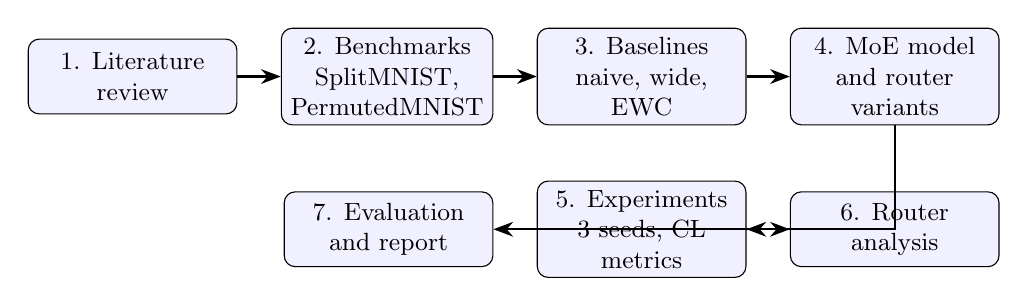
\begin{tikzpicture}[
  pstep/.style={draw, rounded corners, minimum height=0.95cm, minimum width=2.65cm, align=center, fill=blue!6, font=\small},
  arr/.style={-{Stealth[length=2.5mm]}, thick}]
  \node[pstep] (s1) {1. Literature\\review};
  \node[pstep, right=0.55cm of s1] (s2) {2. Benchmarks\\SplitMNIST,\\PermutedMNIST};
  \node[pstep, right=0.55cm of s2] (s3) {3. Baselines\\naive, wide,\\EWC};
  \node[pstep, right=0.55cm of s3] (s4) {4. MoE model\\and router\\variants};
  \node[pstep, below=0.7cm of s3] (s5) {5. Experiments\\3 seeds, CL\\metrics};
  \node[pstep, right=0.55cm of s5] (s6) {6. Router\\analysis};
  \node[pstep, left=0.55cm of s5] (s7) {7. Evaluation\\and report};
  \draw[arr] (s1) -- (s2);
  \draw[arr] (s2) -- (s3);
  \draw[arr] (s3) -- (s4);
  \draw[arr] (s4.south) |- (s5.east);
  \draw[arr] (s5) -- (s6);
  \draw[arr] (s6) -- (s7);
\end{tikzpicture}
\caption{Overview of the approach of this project.}
\label{fig:approach}
\end{figure}

In the first step, the literature on catastrophic forgetting, continual
learning and Mixture of Experts models was studied, and the theoretical
foundation was worked out. This foundation is presented in Chapter~2. In
the second step, the two benchmarks were constructed and the problem was
analysed in detail; this analysis and the resulting requirements are
documented in Chapter~3. In the third and fourth step, the baseline models
and the Mixture of Experts model with its router were designed, which is
the content of Chapter~4. The concrete implementation in Python and
PyTorch is described in Chapter~5. Chapter~6 explains how the implemented
programs were brought into operation and how the experiment suite was
executed. Chapter~7 evaluates the results of all experiments, including a
detailed router analysis and an architecture variant that resulted from the
findings. Chapter~8 finally summarises the achieved results and gives an
outlook on possible extensions.

\chapter{Fundamentals}
\label{chap:fundamentals}

This chapter presents the theoretical knowledge that is needed for the
solution of the problem. Only contents that are used later in the report
are included. Section~2.1 revisits feed forward neural networks and their
training. Section~2.2 formalises continual learning and its standard
scenarios. Section~2.3 explains catastrophic forgetting in more detail, and
Section~2.4 defines the metrics that are used to measure it. Section~2.5
introduces the Mixture of Experts architecture and its gating mechanism.

\section{Feed Forward Neural Networks}
\label{sec:fnn}

An artificial neural network is a parametric function
$f_{\theta} : \mathbb{R}^{d} \rightarrow \mathbb{R}^{c}$ that is built from
layers of simple computational units. A fully connected layer computes
\begin{equation}
  h^{(l)} = \phi\!\left(W^{(l)} h^{(l-1)} + b^{(l)}\right),
  \label{eq:layer}
\end{equation}
where $h^{(l-1)} \in \mathbb{R}^{d_{l-1}}$ is the input of the layer,
$W^{(l)} \in \mathbb{R}^{d_l \times d_{l-1}}$ is the weight matrix,
$b^{(l)} \in \mathbb{R}^{d_l}$ is the bias vector, and $\phi$ is a non
linear activation function. Stacking several such layers gives a multi
layer perceptron (MLP). In this project, the rectified linear unit
$\phi(z) = \max(0, z)$, short ReLU, is used for the hidden layers, because
it is simple, fast and reduces the vanishing gradient problem
\cite{goodfellow2016}.

For a classification problem with $c$ classes, the last layer produces a
vector of logits $z \in \mathbb{R}^{c}$, which is converted into a
probability distribution by the softmax function,
\begin{equation}
  p(y = i \mid x) = \frac{\exp(z_i)}{\sum_{j=1}^{c} \exp(z_j)}.
  \label{eq:softmax}
\end{equation}
The network is trained by minimising the cross entropy loss
\begin{equation}
  \mathcal{L}_{\mathrm{CE}}(\theta)
    = -\frac{1}{N} \sum_{n=1}^{N} \log p(y_n \mid x_n; \theta)
  \label{eq:ce}
\end{equation}
over a training set $\{(x_n, y_n)\}_{n=1}^{N}$ with mini batch stochastic
gradient descent or one of its adaptive variants. In this project, the Adam
optimiser \cite{kingma2015} is used. Adam keeps an estimate of the first
and the second moment of the gradient for every parameter and adapts the
effective step size accordingly, which makes the training robust against a
suboptimal choice of the learning rate.

An important property of such networks for this project is that the
knowledge of the network is stored in a distributed way. Every weight
takes part in the computation of every output, and every output depends on
many weights. This property is one of the main reasons for the forgetting
problem that is described in Section~2.3.

\section{Continual Learning}
\label{sec:cl}

\subsection{Problem Definition}

In continual learning, the training data is not available as one static
data set but arrives as a sequence of $T$ tasks
$\mathcal{T}_1, \mathcal{T}_2, \dots, \mathcal{T}_T$. Each task
$\mathcal{T}_t$ consists of a data set
$\mathcal{D}_t = \{(x_i^{(t)}, y_i^{(t)})\}_{i=1}^{N_t}$
from a task specific distribution. At time $t$, the learner has only access
to $\mathcal{D}_t$, or at most to a very limited memory of earlier tasks,
and has to update its parameters from $\theta_{t-1}$ to $\theta_t$. The
goal is to perform well on all tasks seen so far, not only on the current
one.

This setting is fundamentally different from multi task learning, where the
data of all tasks is available at the same time and can be mixed freely,
and also from transfer learning, where only the performance on a new target
task matters and the performance on the source task is allowed to degrade.

\subsection{The Three Continual Learning Scenarios}
\label{sec:scenarios}

Van de Ven and Tolias \cite{vandeven2019} distinguish three scenarios of
increasing difficulty, which differ in the information that is available at
test time:

\begin{description}[style=nextline]
  \item[Task incremental learning.] The task identity is known at test
        time. The model may use task specific components, for example a
        separate output head per task, and it only has to solve the sub
        problem of the current task. SplitMNIST with one output head per
        task belongs to this scenario.
  \item[Domain incremental learning.] The task identity is not needed at
        test time, but all tasks share the same output space. The model
        must solve every task without knowing which task an input belongs
        to, but it never has to distinguish classes of different tasks.
        PermutedMNIST with one shared ten class head is the standard
        example.
  \item[Class incremental learning.] The model additionally has to infer
        the task identity itself, that is, it has to distinguish all
        classes of all tasks at the same time. This is the hardest of the
        three scenarios.
\end{description}

The two benchmarks of this project cover the first two scenarios. This is a
deliberate choice, as explained in Section~1.2: the main goal is to study
the stability plasticity behaviour of the Mixture of Experts architecture
in a clean setting, not to solve the harder class incremental problem,
which usually needs additional memory based techniques.

\subsection{The Stability Plasticity Dilemma}
\label{sec:dilemma}

Every continual learning method has to balance plasticity, the ability to
gain new knowledge, against stability, the ability to keep old knowledge
\cite{mermillod2013}. Regularisation based methods implement this trade off
explicitly with an additional stability term in the loss function.
Architectural methods implement it implicitly by assigning different parts
of the network to different tasks. The Mixture of Experts approach
investigated here realises the trade off through routing: the plasticity is
concentrated in the experts that the router selects for the new task, while
the remaining experts act as stable memory.

\section{Catastrophic Forgetting}
\label{sec:forgetting}

Catastrophic forgetting denotes the fast and severe loss of previously
learned performance when a neural network is trained on new information.
The phenomenon was documented systematically by McCloskey and Cohen
\cite{mccloskey1989}, who showed that networks trained sequentially on two
lists of associations perform almost at chance level on the first list
after learning the second one. French \cite{french1999} related the effect
to the distributed representations of connectionist models: because all
weights take part in the storage of every pattern, writing a new pattern
into the network inevitably overwrites parts of the old ones.

From the optimisation point of view, the reason is simple. During the
training on task $\mathcal{T}_t$, gradient descent follows the loss
landscape of $\mathcal{L}_t$ only. Nothing in the objective prevents the
parameters from moving to a region of the weight space that is good for
$\mathcal{T}_t$ but arbitrarily bad for the earlier tasks. Because the loss
surfaces of different tasks usually do not share a common minimum in a high
dimensional weight space, sequential optimisation almost guarantees
interference \cite{goodfellow2013}.

It is important to note that catastrophic forgetting is not caused by a
lack of capacity. Even networks with far more parameters than needed for
each single task forget, because the same parameters are reused for all
tasks. This observation is the key motivation for the present project: a
Mixture of Experts model can partition its capacity so that different tasks
rely on different parameters, and can therefore attack the root cause of
the interference instead of only dampening its symptoms.

\section{Metrics for Continual Learning}
\label{sec:clmetrics}

To make forgetting measurable, the evaluation follows the standard protocol
of Lopez-Paz and Ranzato \cite{lopezpaz2017}. Let
\begin{equation}
  R_{i,j} \in [0,1]
\end{equation}
be the test accuracy on task $\mathcal{T}_j$ after the model has been
trained on task $\mathcal{T}_i$, with $j \leq i$. The triangular matrix $R$
describes the complete learning dynamic of a run. Three scalar metrics are
derived from it.

The average accuracy is the mean performance over all tasks after the last
training stage,
\begin{equation}
  A = \frac{1}{T} \sum_{j=1}^{T} R_{T,j}.
  \label{eq:avgacc}
\end{equation}
It reflects plasticity and stability together and is the primary metric of
a continual learner.

The average forgetting measures, for every task, the difference between the
best accuracy ever reached on it and its accuracy at the end of training:
\begin{equation}
  F = \frac{1}{T-1} \sum_{j=1}^{T-1}
      \Big( \max_{i \in \{j, \dots, T-1\}} R_{i,j} - R_{T,j} \Big).
  \label{eq:forgetting}
\end{equation}
A value of $F = 0$ means perfect retention; larger positive values mean
more severe forgetting.

The backward transfer (BWT) measures the average influence that learning a
new task has on the performance on previous tasks,
\begin{equation}
  \mathrm{BWT} = \frac{1}{T-1} \sum_{j=1}^{T-1} \left( R_{T,j} - R_{j,j} \right).
  \label{eq:bwt}
\end{equation}
Negative values indicate forgetting; positive values would mean that
learning later tasks even improved the earlier ones.

\section{Mixture of Experts}
\label{sec:moe}

\subsection{Historical Roots}

The Mixture of Experts idea goes back to Jacobs, Jordan, Nowlan and
Hinton \cite{jacobs1991}, who proposed to replace one single network by a
set of expert networks together with a gating network. Each expert
specialises on a region of the input space, and the gating network learns
to assign every input to the most suitable expert. Because the experts are
trained jointly but compete through the gate, the architecture shows a
form of divide and conquer: a complex problem is decomposed into simpler
sub problems that are solved by specialists. Hierarchical variants of the
model were analysed afterwards by Jordan and Jacobs \cite{jordan1994}.

\subsection{Sparsely Gated Mixture of Experts}
\label{sec:sparsemoe}

The modern, scalable form of the idea is the sparsely gated MoE layer of
Shazeer et al.\ \cite{shazeer2017}. Instead of weighting all experts, the
gate activates only the $k$ best ones, typically $k \in \{1, 2\}$, which
keeps the computational cost per input almost constant while the total
number of parameters grows with the number of experts. This architecture
later became a core component of very large language models, most notably
the Switch Transformer \cite{fedus2022}, and showed that expert based
capacity scaling works reliably in practice.

Formally, an MoE layer consists of $E$ expert networks $f_1, \dots, f_E$
and a gating network $g$. For an input $h$, the gate first computes logits
and converts them into a probability distribution over the experts:
\begin{equation}
  g(h) = \mathrm{softmax}\!\left(W_g h + b_g\right) \in \mathbb{R}^{E}.
  \label{eq:gate}
\end{equation}
Only the $k$ experts with the largest gate values are evaluated. If
$\mathcal{S}(h) = \operatorname{top}\text{-}k\big(g(h)\big)$ denotes the
index set of the selected experts and $\tilde{g}_e$ their renormalised gate
values, the output of the layer is the convex combination
\begin{equation}
  \mathrm{MoE}(h) = \sum_{e \in \mathcal{S}(h)} \tilde{g}_e(h) \, f_e(h),
  \qquad
  \tilde{g}_e(h) = \frac{g_e(h)}{\sum_{e' \in \mathcal{S}(h)} g_{e'}(h)}.
  \label{eq:moe}
\end{equation}
All parameters, those of the experts and those of the gate, are trained
jointly by backpropagation; the gate receives gradients through the weights
$\tilde{g}_e$.

\subsection{Load Balancing}
\label{sec:loadbalance}

A well known failure mode of MoE training is expert collapse: the gate
quickly prefers one or two experts, these experts receive more gradient
signal and become even better, and the remaining experts starve. To prevent
this, an auxiliary loss is used that rewards a uniform usage of the experts
\cite{shazeer2017}. The variant used in this project follows the Switch
Transformer \cite{fedus2022}. Let $f_e$ be the fraction of samples of a
batch whose highest ranked expert is $e$, and let $P_e$ be the mean gate
probability of expert $e$ over the batch. Then
\begin{equation}
  \mathcal{L}_{\mathrm{LB}} = E \cdot \sum_{e=1}^{E} f_e \, P_e
  \label{eq:lb}
\end{equation}
is minimised when all experts are used equally. It is added to the task
loss with a small coefficient $\alpha$:
\begin{equation}
  \mathcal{L} = \mathcal{L}_{\mathrm{CE}} + \alpha \, \mathcal{L}_{\mathrm{LB}}.
  \label{eq:totalloss}
\end{equation}
As Chapter~7 will show, this auxiliary loss has an unexpected and important
side effect in the continual setting.

\subsection{Position of the MoE Layer in the Network}
\label{sec:moeposition}

A design question that is rarely discussed in the MoE literature, but is
central for this project, is where in the network the MoE layer should be
placed. In large language models, the MoE layers replace the feed forward
blocks in the middle of a deep stack, so the router always sees a hidden
representation that was produced by shared layers in front of it. Two
extreme positions can be distinguished.

With \emph{hidden level routing}, the input first passes one or more shared
layers, and the router assigns the resulting hidden representation to the
experts. The shared layers form a common feature extractor for all inputs,
and the experts only specialise on the later processing stages. With
\emph{input level routing}, the router and the experts act directly on the
raw input, and only the mixed expert output passes shared layers.

The difference matters for continual learning, because routing can only
protect the parameters that lie behind the router. Parameters in front of
the router process every input of every task and are updated by every
task, so they behave exactly like the weights of a dense network. If two
tasks differ in the way the raw input must be interpreted, as for example
two different pixel permutations do, the decisive task specific knowledge
lives precisely in this early mapping. A router behind a shared trunk
cannot protect this mapping, no matter how well it separates the tasks in
the hidden space. This consideration is taken up again in the design
decisions of Chapter~4 and becomes directly relevant in the evaluation in
Chapter~7.

\subsection{Why MoE Is Attractive for Continual Learning}
\label{sec:whymoe}

The connection between MoE and continual learning is the central idea of
this project. Three properties make the architecture promising. First,
conditional computation: only a subset of the network is active for any
given input, so if the router separates tasks, the gradient updates on a
new task touch only a subset of the parameters, which directly limits
interference. Second, spare capacity: the total number of parameters scales
with the number of experts, not with the cost per input, so new tasks can
occupy capacity that was not needed by earlier tasks. Third, learned task
inference: the gate itself is a small classifier that learns, without being
told the task identity, to distinguish the input distributions of the
tasks. Whether these properties actually appear in a sequential training
regime, and how strongly they protect against forgetting, is exactly what
the experiments in Chapter~7 are designed to measure.

\chapter{Problem Analysis}
\label{chap:analysis}

The analysis of the problem to be solved is the basis of every engineering
like procedure. In this chapter, the overall problem is decomposed into sub
problems on the basis of the fundamentals of Chapter~2, the existing
solution approaches from the literature are analysed, and the requirements
for the system to be developed are derived.

\section{Decomposition of the Problem}
\label{sec:decomposition}

The overall problem, learning a sequence of tasks without losing old
knowledge, can be decomposed into the following sub problems:

\begin{enumerate}[label=\textbf{SP\arabic*.}, leftmargin=3em]
  \item \textbf{Representation of knowledge.} In which part of the network
        is the knowledge about a task stored, and how can new knowledge be
        added without changing the old one?
  \item \textbf{Assignment of tasks to parameters.} Which parameters should
        be updated when a new task arrives, and who makes this decision?
  \item \textbf{Measurement of forgetting.} How can forgetting be measured
        objectively, so that different solutions can be compared fairly?
  \item \textbf{Fair comparison.} How can it be guaranteed that an observed
        improvement comes from the investigated mechanism and not, for
        example, simply from a larger number of parameters?
\end{enumerate}

These sub problems depend on each other. The assignment of tasks to
parameters (SP2) decides directly about the representation of knowledge
(SP1): if two tasks share all parameters, interference is unavoidable, as
explained in Section~2.3. The measurement (SP3) is needed before any
solution can be judged, and the fairness question (SP4) decides which
baseline models the experiment needs. The design in Chapter~4 answers SP1
and SP2 with the Mixture of Experts architecture and its router, while the
experiment protocol in Chapters~6 and~7 answers SP3 and SP4.

\section{Analysis of Existing Solution Approaches}
\label{sec:existing}

Continual learning has been studied intensively in the last years, and
several surveys give a systematic overview
\cite{delange2021,wang2024survey,masana2022}. The existing methods can be
divided into three families.

\subsection{Regularisation Based Methods}

Regularisation based methods leave the network architecture unchanged and
modify the loss function instead. The most influential representative is
Elastic Weight Consolidation (EWC) \cite{kirkpatrick2017}. After finishing
a task, EWC estimates the importance of every parameter by the diagonal of
the Fisher information matrix,
\begin{equation}
  F_{ii} = \mathbb{E}\!\left[\left(
    \frac{\partial \log p(y \mid x; \theta)}{\partial \theta_i}
  \right)^{2}\right],
  \label{eq:fisher}
\end{equation}
and afterwards punishes quadratic deviations of important parameters from
their stored values $\theta_i^{*}$:
\begin{equation}
  \mathcal{L}_{\mathrm{EWC}}(\theta)
    = \mathcal{L}_{t}(\theta)
      + \frac{\lambda}{2} \sum_{i} F_{ii}\,(\theta_i - \theta_i^{*})^{2}.
  \label{eq:ewc}
\end{equation}
The coefficient $\lambda$ controls the stability plasticity trade off.
Related methods estimate the importance differently: Synaptic Intelligence
accumulates an online importance measure along the optimisation path
\cite{zenke2017}, and Memory Aware Synapses estimates the importance from
the sensitivity of the output function \cite{aljundi2018}. A shared
limitation is that the quadratic penalty is only a local approximation:
with more and more tasks, the collected constraints can rigidify the
network and finally prevent it from learning new tasks at all. A second
branch of regularisation avoids storing old data by distillation, for
example Learning without Forgetting \cite{li2017}.

\subsection{Replay Based Methods}

Replay methods keep a small episodic memory of real or generated samples
from earlier tasks and mix them into the training of new tasks. iCaRL
\cite{rebuffi2017} combines an exemplar memory with a nearest mean
classifier. Gradient Episodic Memory \cite{lopezpaz2017} uses the memory to
constrain the gradient updates so that the loss on every remembered task
cannot increase. Generative replay replaces the stored samples with data
from a learned generative model \cite{shin2017}. Replay belongs to the
strongest strategies, but it needs to store data, which can be impossible
for privacy reasons, and the memory grows with the number of tasks.

\subsection{Architecture Based Methods}

The third family changes the network itself. Progressive Neural Networks
\cite{rusu2016} allocate a new network column per task and connect it to
the frozen columns of earlier tasks; forgetting is impossible by
construction, but the number of parameters grows linearly with the number
of tasks, and the task identity must be known at test time. Other
approaches assign a binary mask to every task and train only the unmasked
weights \cite{mallya2018}. Expert Gate \cite{aljundi2017} is conceptually
closest to this project: it also uses a network of experts with a gating
mechanism, but it trains one new expert per task and selects experts by the
task identity, while the approach here lets the router learn the assignment
fully automatically without any task labels.

\subsection{Comparison of the Method Families}

Table~3.1 contrasts the three families along the criteria that matter for
this project. No family dominates the others. Regularisation methods are
cheap and need neither stored data nor task labels, but their protection is
only a local approximation of the true loss landscape, and the accumulated
constraints of many tasks can finally block further learning. Replay
methods reach the strongest results in most benchmarks, but they store old
data or a generative model of old data, which can be impossible under
privacy constraints, and their memory requirement grows with the length of
the task sequence. Architectural methods avoid both problems, but the
existing representatives either grow the network with every task or need
the task identity at test time to select the right component.

\begin{table}[H]
  \centering
  \small
  \caption{Comparison of the three continual learning method families.}
  \label{tab:families}
  \begin{tabular}{lccc}
    \toprule
    \textbf{Criterion} & \textbf{Regularisation} & \textbf{Replay} & \textbf{Architecture} \\
    \midrule
    Stores old data          & no   & yes  & no \\
    Needs task identity      & no   & no   & often \\
    Capacity growth per task & none & memory only & often linear \\
    Protection mechanism     & approximate & strong & structural \\
    Representative methods   & EWC, SI, MAS & iCaRL, GEM & PNN, Expert Gate \\
    \bottomrule
  \end{tabular}
\end{table}

For the present project, the decisive criterion is the combination of the
first three rows: a method that stores no data, needs no task labels and
does not grow without limit. Only a softly partitioned architecture can
offer all three properties at the same time. A Mixture of Experts model
with a learned router is a natural candidate, because its capacity is
fixed in advance but is used conditionally, so new tasks can occupy experts
that earlier tasks rarely touch.

\subsection{Conclusion for this Project}

The analysis shows a gap: regularisation methods are efficient but only
approximate, replay methods are strong but need stored data, and existing
architectural methods either grow without limit or need the task identity.
A Mixture of Experts model with a learned router promises a middle way: no
stored data, no task labels, and a capacity that is partitioned softly
instead of being fixed by hand. This promise is tested in the present
project.

\section{Requirements Analysis}
\label{sec:requirements}

From the problem analysis, the following requirements for the system were
collected and prioritised in four categories, as it is common practice for
project work.

\paragraph{Must have requirements.}
\begin{itemize}[leftmargin=2em]
  \item \textbf{M1:} Sequential training of a model on a sequence of tasks
        without access to the data of earlier tasks.
  \item \textbf{M2:} At least two continual learning benchmarks built from
        MNIST (SplitMNIST and PermutedMNIST).
  \item \textbf{M3:} A working Mixture of Experts model with a trainable
        router and more than two experts.
  \item \textbf{M4:} A naive baseline with the same training protocol for
        comparison.
  \item \textbf{M5:} Quantitative evaluation with the standard metrics
        average accuracy, average forgetting and backward transfer after
        every training stage.
\end{itemize}

\paragraph{Should have requirements.}
\begin{itemize}[leftmargin=2em]
  \item \textbf{S1:} A regularisation baseline (EWC) to position the MoE
        results relative to an established method.
  \item \textbf{S2:} A capacity matched wide baseline to separate capacity
        effects from routing effects (answers SP4).
  \item \textbf{S3:} Reproducibility through fixed random seeds and
        repeated runs.
  \item \textbf{S4:} Analysis of the router (expert usage per task).
\end{itemize}

\paragraph{Could have requirements.}
\begin{itemize}[leftmargin=2em]
  \item \textbf{C1:} An auxiliary loss for load balancing that keeps all
        experts active.
  \item \textbf{C2:} Configurable hyperparameters (number of experts, top
        $k$, epochs, learning rate).
\end{itemize}

\paragraph{Nice to have requirements.}
\begin{itemize}[leftmargin=2em]
  \item \textbf{N1:} Extension to further benchmarks or to the class
        incremental scenario.
  \item \textbf{N2:} Dynamic addition of new experts per task.
\end{itemize}

All must have and should have requirements were realised, and C1 and C2
were realised as well. N1 and N2 remain future work and are discussed in
Section~8.2.

\chapter{Solution Concept}
\label{chap:concept}

On the basis of the problem analysis of Chapter~3 and the theoretical
knowledge of Chapter~2, this chapter develops the solution concept.
Section~4.1 gives an overview of the system architecture. Section~4.2
specifies the Mixture of Experts model, Section~4.3 the router, and
Section~4.4 the continual training procedure.

\section{Architectural Overview}
\label{sec:overview}

The system is organised in four loosely coupled layers, which are shown in
Figure~4.1 together with their data flow.

\begin{figure}[H]
\centering
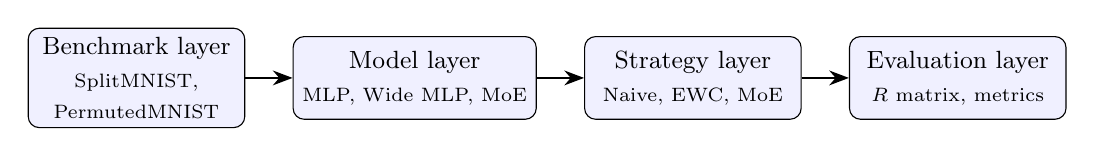
\begin{tikzpicture}[
  box/.style={draw, rounded corners, minimum height=1.05cm, minimum width=2.75cm, align=center, fill=blue!6, font=\small},
  arr/.style={-{Stealth[length=2.5mm]}, thick}]
  \node[box] (data) {Benchmark layer\\[1pt] \scriptsize SplitMNIST,\\ \scriptsize PermutedMNIST};
  \node[box, right=0.6cm of data] (model) {Model layer\\[1pt] \scriptsize MLP, Wide MLP, MoE};
  \node[box, right=0.6cm of model] (train) {Strategy layer\\[1pt] \scriptsize Naive, EWC, MoE};
  \node[box, right=0.6cm of train] (eval) {Evaluation layer\\[1pt] \scriptsize $R$ matrix, metrics};
  \draw[arr] (data) -- (model);
  \draw[arr] (model) -- (train);
  \draw[arr] (train) -- (eval);
\end{tikzpicture}
\caption{Layered concept of the experimental system. The data flows from
the benchmark layer through the model and strategy layers to the evaluation
layer, which produces the accuracy matrix, the scalar metrics and the
router profiles.}
\label{fig:system}
\end{figure}

The benchmark layer turns a static data set into a sequence of tasks and
provides one training and one test data loader per task. The model layer
contains the network architectures: the baseline MLP, the wide MLP and the
Mixture of Experts network. The strategy layer implements the training
procedures, namely naive fine tuning, EWC and the MoE training with the
auxiliary loss. Finally, the evaluation layer computes the accuracy matrix
$R$ after every training stage, derives the scalar metrics from it and
extracts the router profiles for the MoE model.

This separation had two practical advantages during the project. First,
every component could be implemented and tested independently. Second, the
comparison between the approaches stays fair, because all approaches
consume exactly the same task sequence and are evaluated by exactly the
same code. This directly answers the fairness sub problem SP4 of
Section~3.1.

\section{Concept of the MoE Model}
\label{sec:moedesign}

The proposed model follows the structure sketched in Figure~4.2. A shared
trunk maps the flattened $28 \times 28$ input image to a $400$ dimensional
representation. This representation is processed by one MoE layer
consisting of $E = 8$ experts and a router. Each expert is a small feed
forward block with one hidden layer and ReLU activation, with identical
input and output dimension, so that the expert outputs can be combined by a
weighted sum. The router selects the $k = 2$ experts with the highest gate
values for every sample and combines their outputs according to
Equation~\eqref{eq:moe}. On top of the MoE layer, one linear output head
per task produces the class logits (multi head protocol, see
Section~2.2.2).

\begin{figure}[H]
\centering
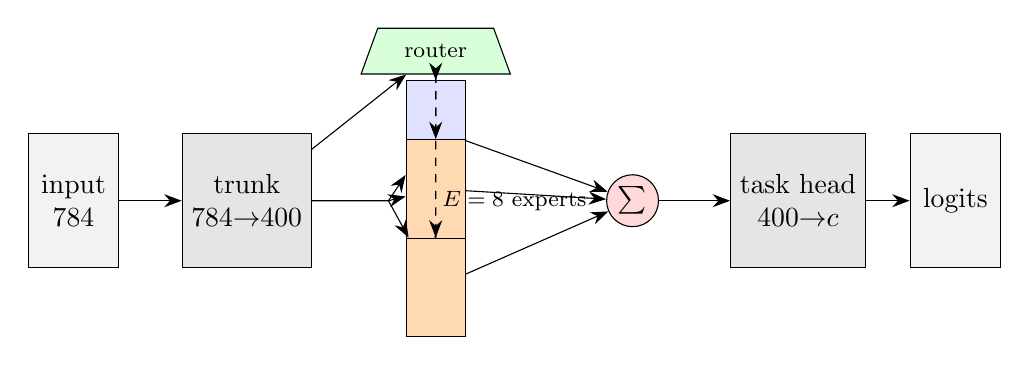
\begin{tikzpicture}[
  x=1cm, y=1cm,
  io/.style={draw, minimum width=1.15cm, minimum height=1.7cm, fill=gray!10, align=center},
  exp/.style={draw, minimum width=0.75cm, minimum height=1.25cm, fill=blue!12},
  expa/.style={draw, minimum width=0.75cm, minimum height=1.25cm, fill=orange!30},
  router/.style={draw, trapezium, trapezium angle=70, minimum width=1.9cm, fill=green!15, align=center},
  sum/.style={draw, circle, inner sep=1.5pt, fill=red!15},
  arr/.style={-{Stealth[length=2.2mm]}}]
  \node[io] (in) at (0,0) {input\\ $784$};
  \node[io, fill=gray!20] (trunk) at (2.2,0) {trunk\\ $784{\rightarrow}400$};
  \node[router] (gate) at (4.6,1.9) {\footnotesize router};
  \node[exp]  (e1) at (4.6,0.9) {};
  \node[expa] (e2) at (4.6,0.15) {};
  \node at (4.6,-0.5) {\footnotesize $\vdots$};
  \node[expa] (e8) at (4.6,-1.1) {};
  \node at (5.6,0) {\footnotesize $E=8$ experts};
  \node[sum] (plus) at (7.1,0) {$\sum$};
  \node[io, fill=gray!20] (head) at (9.2,0) {task head\\ $400{\rightarrow}c$};
  \node[io] (out) at (11.2,0) {logits};
  \draw[arr] (in) -- (trunk);
  \draw[arr] (trunk) -- (gate);
  \draw[arr] (trunk) -- (4.0,0) -- (e1);
  \draw[arr] (4.0,0) -- (e2);
  \draw[arr] (4.0,0) -- (e8);
  \draw[arr,dashed] (gate) -- (e1);
  \draw[arr,dashed] (gate) -- (e2);
  \draw[arr,dashed] (gate) -- (e8);
  \draw[arr] (e1) -- (plus);
  \draw[arr] (e2) -- (plus);
  \draw[arr] (e8) -- (plus);
  \draw[arr] (plus) -- (head);
  \draw[arr] (head) -- (out);
\end{tikzpicture}
\caption{Concept of the MoE model. A shared trunk feeds eight parallel
experts. The router (dashed arrows) selects the top 2 experts per sample
(highlighted); their outputs are combined as a gate weighted sum and passed
to the output head of the current task.}
\label{fig:moearch}
\end{figure}

The choice $E = 8$ with $k = 2$ follows the efficiency requirement of
Section~1.2: with five tasks, eight experts give enough spare capacity for
the router to separate the tasks, while the activated computation per
sample, namely two experts, stays close to that of the baseline. The output
head per task keeps the comparison with the baselines protocol fair,
because the baselines use identical heads.

\section{Concept of the Router}
\label{sec:routerdesign}

The router is a single linear layer $W_g \in \mathbb{R}^{8 \times 400}$
followed by a softmax, see Equation~\eqref{eq:gate}. It is deliberately
kept simple: a small gate cannot itself become a bottleneck of forgetting,
and its decisions stay easy to interpret and to visualise. Two design
decisions are essential for the continual setting:

\begin{enumerate}[label=\textbf{D\arabic*.}, leftmargin=3em]
  \item The router does not receive the task identity. The gate only sees
        the hidden representation of the input. Every task separation it
        shows is therefore learned from the data alone, which makes the
        router analysis in Chapter~7 meaningful.
  \item The router is trained only on the current task, without any
        mechanism that forces it to keep old routing decisions. If the
        gate changed its assignments freely, previously acquired expert
        knowledge would be re-routed and lost. The experiments test whether
        the assignments stay stable enough in practice.
\end{enumerate}

The auxiliary loss for load balancing from Equation~\eqref{eq:lb}, with the
coefficient $\alpha = 0.01$, prevents expert collapse at the beginning of
training and guarantees that all eight experts stay functional, so that
later tasks can actually find unused capacity. As the evaluation will show,
this component behaves differently than expected in the continual setting,
which leads to the architecture variant described in Section~7.5.

\paragraph{Considered alternatives.} Two alternative router designs were
considered and rejected. The first alternative was a nonlinear gate with
one hidden layer. It was rejected because the gate itself is part of the
continual learning problem: a larger gate has more parameters that can
forget, and its decisions are harder to interpret in the router analysis.
The second alternative was a hard top one routing without any mixing,
as in the Switch Transformer \cite{fedus2022}. It was rejected for this
small scale setting because the gradient signal of a single expert per
sample is noisy, and because a soft mixing of two experts makes the
transition between tasks smoother when the router changes its assignment.
The top two choice keeps most of the sparsity but keeps training stable,
which was confirmed in preliminary tests.

\paragraph{Expected behaviour.} If the concept works as intended, the
following behaviour should be observable in the experiments. During the
first task, the router distributes the samples over several experts. When
the second task arrives, the router should prefer experts that carry little
knowledge of the first task, so that the gradient updates of the new task
mainly rewrite unused or weakly used parameters. Over the whole sequence,
a pattern of task specific expert subsets should emerge, and the pairwise
routing similarity between tasks should stay low. These predictions are
checked explicitly in Section~7.6.

\section{Concept of the Training Procedure}
\label{sec:trainingdesign}

All approaches follow the same sequential protocol, which is shown in
Table~4.1. For every task, the model is trained from its current state on
the training data of that task; afterwards, it is evaluated on the test
data of all tasks seen so far, which produces one row of the accuracy
matrix $R$. No data of earlier tasks is shown again, and no task boundaries
are signalled to the router.

\begin{table}[H]
\centering
\caption{Sequential continual training protocol used for all approaches.}
\label{tab:protocol}
\begin{tabular}{p{0.86\textwidth}}
\toprule
\textbf{Algorithm:} Sequential training over a task sequence \\
\midrule
\textbf{Input:} task sequence $(\mathcal{T}_1, \dots, \mathcal{T}_T)$;
model $f_\theta$; strategy specific loss $\mathcal{L}$ \\
1: \textbf{for} $t = 1$ \textbf{to} $T$ \textbf{do} \\
2: \quad train $f_\theta$ on $\mathcal{T}_t$ by minimising $\mathcal{L}$ \\
3: \quad \textbf{for} $j = 1$ \textbf{to} $t$ \textbf{do} \\
4: \quad \quad $R_{t,j} \leftarrow$ accuracy of $f_\theta$ on the test set of $\mathcal{T}_j$ \\
5: \quad \textbf{end for} \\
6: \textbf{end for} \\
7: derive $A$, $F$ and BWT from $R$ (Equations \eqref{eq:avgacc} to \eqref{eq:bwt}) \\
\bottomrule
\end{tabular}
\end{table}

For the EWC strategy, step 2 additionally estimates the diagonal Fisher
information on the current task after convergence and accumulates the
quadratic penalty of Equation~\eqref{eq:ewc} for all later tasks. For the
MoE strategy, step 2 minimises the combined loss of
Equation~\eqref{eq:totalloss}. The evaluation in lines 3 to 5 is identical
for all approaches, which guarantees that differences in the metrics can be
attributed to the models and strategies alone.

\chapter{Implementation}
\label{chap:implementation}

This chapter describes the concrete implementation of the solution concept
from Chapter~4. Section~5.1 lists the used development tools,
Section~5.2 describes the module structure of the code, and
Sections~5.3 to~5.5 explain the implementation of the benchmarks, the
models and the training strategies. Only one short code excerpt is shown;
the complete source code is printed in Appendix~A.

\section{Development Tools}
\label{sec:stack}

The system was implemented in Python~3.12. As deep learning framework,
PyTorch~2.8 \cite{paszke2019} with torchvision for data loading was used.
NumPy was used for numerical post processing and Matplotlib for the
visualisation of the results. All experiments ran on the CPU of a standard
Linux machine; no GPU was necessary, because the models and data sets are
small. Every module is documented by docstrings and inline comments.

\section{Module Structure}
\label{sec:implstructure}

The code is organised as a small package with one module per layer of the
concept in Figure~4.1:

\begin{itemize}[leftmargin=2em]
  \item \texttt{datasets.py}: construction of the SplitMNIST and
        PermutedMNIST task sequences (benchmark layer);
  \item \texttt{models.py}: the baseline MLP, the wide MLP, the MoE network
        and the input level MoE variant (model layer);
  \item \texttt{continual.py}: the training strategies naive, EWC and MoE,
        together with the evaluation metrics (strategy and evaluation
        layer);
  \item \texttt{run\_experiments.py}, \texttt{run\_ablation.py} and
        \texttt{run\_v2.py}: the experiment drivers for the main
        experiments, the load balancing ablation and the architecture
        variant;
  \item \texttt{make\_figures.py} and \texttt{make\_tables.py}: generation
        of all figures and result tables of this report directly from the
        stored results.
\end{itemize}

\section{Benchmark Construction}
\label{sec:implbench}

\subsection{SplitMNIST}

The ten MNIST classes are split into five consecutive tasks
$\{0,1\}, \{2,3\}, \dots, \{8,9\}$. For every task, the samples of the two
classes are extracted from the original training and test sets, the labels
are remapped to the local classes $\{0,1\}$ of the task specific output
head, and the images are flattened to vectors of $784$ float values. The
result is a task incremental benchmark in the multi head protocol of
Section~2.2.2.

\subsection{PermutedMNIST}

For PermutedMNIST, the first task is the original MNIST data set. For every
later task, a fixed random permutation of the $784$ pixel positions is
drawn from a seeded random number generator and applied to all images of
that task. Because the classes stay the same in every task, all tasks share
one ten class output head, which realises the domain incremental scenario.
The permutation is applied on the fly when a sample is loaded, so the base
tensors are stored only once and the memory usage stays low even for many
tasks.

\section{Model Implementations}
\label{sec:implmodels}

The baseline network is a two hidden layer MLP with
$784 \rightarrow 400 \rightarrow 400$ units and ReLU activations, plus one
linear output head per task. The wide baseline increases the hidden
dimension to $1100$, which raises its parameter count slightly above the
MoE model and thereby implements the capacity control required in
Section~3.3. Table~5.1 lists the resulting parameter counts.

\begin{table}[H]
  \centering
  \caption{Trainable parameters of the compared architectures (with five
  output heads on SplitMNIST).}
  \label{tab:params}
  \begin{tabular}{lr}
    \toprule
    \textbf{Architecture} & \textbf{Parameters} \\
    \midrule
    Baseline MLP ($784{\rightarrow}400{\rightarrow}400$) & 476{,}004 \\
    MoE, hidden level routing ($8$ experts, top $2$)     & 1{,}602{,}012 \\
    MoE, input level routing ($8$ experts, top $2$)      & 1{,}679{,}752 \\
    Wide MLP ($784{\rightarrow}1100{\rightarrow}1100$)    & 2{,}074{,}600 \\
    \bottomrule
  \end{tabular}
\end{table}

The core of the project is the MoE layer. Listing~5.1 shows its forward
pass. The router computes a softmax distribution over the eight experts,
the two largest gate values are renormalised, and only the selected experts
are evaluated. The outputs are added with their gate values as weights. The
input level variant, which resulted from the evaluation in Chapter~7, uses
the same gating mechanics but places the router and the experts directly at
the raw input instead of behind the shared trunk.

\begin{lstlisting}[caption={Forward pass of the sparsely gated MoE layer
(excerpt from \texttt{models.py}).}, label={lst:moelayer}]
def forward(self, x):
    # compute the gate distribution over all experts
    logits = self.router(x)
    gates = F.softmax(logits, dim=-1)
    topv, topi = gates.topk(self.top_k, dim=-1)
    topv = topv / topv.sum(dim=-1, keepdim=True)

    # evaluate only the selected experts and mix their outputs
    out = torch.zeros_like(x)
    for slot in range(self.top_k):
        idx = topi[:, slot]
        w = topv[:, slot].unsqueeze(1)
        for e in range(self.n_experts):
            mask = idx == e
            if mask.any():
                out[mask] += w[mask] * self.experts[e](x[mask])
    return out, gates
\end{lstlisting}

\section{Training Strategies}
\label{sec:implstrategies}

\subsection{Naive Fine Tuning}

The naive trainer minimises the cross entropy loss of
Equation~\eqref{eq:ce} with the Adam optimiser, learning rate $10^{-3}$,
for five epochs per task. It deliberately does nothing to protect old
knowledge and therefore measures the amount of forgetting that every
continual learning mechanism has to beat.

\subsection{Elastic Weight Consolidation}

The EWC trainer extends the naive trainer in two places. After finishing a
task, it estimates the diagonal Fisher information of
Equation~\eqref{eq:fisher} from the gradients on the training data of that
task and stores a copy of the current parameters. During every later task,
the quadratic penalty of Equation~\eqref{eq:ewc} with $\lambda = 500$ is
added to the loss. The penalty accumulates over tasks, so that all previous
tasks are protected at the same time. Care had to be taken with the lazily
created output heads: heads of other tasks do not take part in the current
computation graph, so their Fisher contribution is skipped.

\subsection{MoE Training}

The MoE trainer minimises the combined loss of
Equation~\eqref{eq:totalloss} with the same optimiser settings as the other
strategies. After the complete task sequence has been learned, it extracts
the router profile: the mean gate probability of every expert, computed
over the test set of every task. This $5 \times 8$ matrix is the raw
material for the router analysis in Section~7.6.

\section{Experiment Drivers and Result Storage}
\label{sec:impldrivers}

Three driver scripts connect the modules to complete experiments. The main
driver \texttt{run\_experiments.py} trains all four approaches on both
benchmarks with three seeds each. Before every run, the random seed is set
explicitly, so that the initialisation of every model and the data order
are identical across approaches and repeatable across machines. After every
single run, the accuracy matrix, the derived metrics, the parameter count
and the runtime are appended to the result file, and the router profile is
stored as a separate NumPy archive. The results are written to disk after
every run instead of only at the end, so a crash or an out of memory stop
cannot destroy the measurements that were already collected. This design
decision proved its value during commissioning, as Section~6.2 describes.

The second driver \texttt{run\_ablation.py} repeats the MoE training on
PermutedMNIST with smaller load balancing coefficients, and the third
driver \texttt{run\_v2.py} evaluates the input level architecture variant
on both benchmarks. All three drivers share the same trainer and metric
code, so the results are directly comparable.

A deliberate property of the implementation is that no number in this
report was copied by hand. The two scripts \texttt{make\_figures.py} and
\texttt{make\_tables.py} read the stored result files and generate every
figure of Chapter~7 as a vector graphic and every result table as a LaTeX
file with the measured values. This closes the gap between the experiment
and the document and removes a common source of transcription errors.

\chapter{Commissioning}
\label{chap:commissioning}

The task of this chapter is to show how the implemented solution was
brought into operation. For this project, this means the preparation of the
runtime environment, the execution of the experiment suite, and the steps
taken to make the results reproducible.

\section{Preparation of the Environment}
\label{sec:environment}

The experiments were carried out on a standard Linux machine with a CPU
only installation. The environment consists of Python~3.12 with the
packages PyTorch~2.8, torchvision, NumPy and Matplotlib. The MNIST raw
files were downloaded once from the official mirror and stored in the
project folder, so that the experiments can run without further downloads.
The installation and execution requires only the following commands:

\begin{lstlisting}[language=bash, caption={Installation and execution of
the experiment suite.}, label={lst:commands}]
pip install torch torchvision numpy matplotlib
cd moe_continual_learning/src
python3 run_experiments.py   # main experiment suite
python3 run_ablation.py      # load balancing ablation
python3 run_v2.py            # input level architecture variant
python3 make_figures.py      # figures for the report
python3 make_tables.py       # LaTeX tables for the report
\end{lstlisting}

\section{Execution of the Experiments}
\label{sec:execution}

The main experiment driver runs the full comparison matrix: four approaches
(naive MLP, MLP with EWC, wide MLP, MoE), two benchmarks (SplitMNIST and
PermutedMNIST) and three random seeds, which results in 24 complete
continual training runs. Before the construction of every model, the global
random seed is reset, so that all approaches start from comparable initial
conditions; the task permutations of PermutedMNIST are also derived from
the seed. After every training stage, the current accuracy row is printed
and stored, so the progress can be followed in the log file. A typical log
line looks as follows:

\begin{lstlisting}[caption={Example lines of the experiment log.},
label={lst:log}]
[split_mnist] seed=0 MoE: avg_acc=0.9523 forgetting=0.0561 bwt=-0.0561
[permuted_mnist] seed=2 MLP + EWC: avg_acc=0.9490 forgetting=0.0354
\end{lstlisting}

The results are written to disk after every single run. This proved to be
important in practice: during the project, one experiment process was
terminated by the operating system because of high memory usage, and thanks
to the incremental storage, no completed run had to be repeated. After this
incident, the PermutedMNIST loader was changed to apply the permutation on
the fly instead of materialising a copy of the whole data set per task,
which reduced the memory consumption of the benchmark clearly.

The runtime of a single continual training run over five tasks lies between
$18\,\mathrm{s}$ (naive MLP on SplitMNIST) and $430\,\mathrm{s}$ (MoE on
PermutedMNIST) on the CPU. The complete main suite takes about one hour,
the ablation about 20 minutes and the architecture variant about 25
minutes.

\section{Reproducibility Measures}
\label{sec:reproducibility}

Several measures were taken so that every number in this report can be
traced back to a concrete training run. All random choices are controlled
by seeds: the initialisation of every model, the data order of every
training run and the pixel permutations of PermutedMNIST. As a consequence,
repeated executions of the suite produce identical results, which was
verified explicitly when the suite had to be restarted after the incident
described above. The raw results of every run are stored as JSON files, and
the router profiles are stored separately as compressed NumPy archives.
Finally, all figures and all result tables of Chapter~7 were generated
directly from these stored results by the two scripts
\texttt{make\_figures.py} and \texttt{make\_tables.py}; no number was
copied by hand.

\chapter{Evaluation}
\label{chap:evaluation}

The task of the evaluation is to check to what extent the objectives of the
work were reached. Section~7.1 describes the experimental setup,
Sections~7.2 and~7.3 report the results on SplitMNIST and PermutedMNIST,
Section~7.4 analyses why the first MoE architecture fails on PermutedMNIST,
Section~7.5 evaluates the resulting architecture variant, Section~7.6
analyses the behaviour of the router, and Section~7.7 discusses the
findings.

\section{Experimental Setup}
\label{sec:setup}

Both benchmarks consist of five tasks and were constructed exactly as
described in Section~5.3. SplitMNIST is evaluated in the task incremental
multi head protocol, PermutedMNIST in the domain incremental protocol with
one shared ten class head. All approaches see the identical task sequence,
the identical data order and the identical pixel permutations, because all
random choices are derived from controlled seeds.

Four approaches are compared in the main experiment: the naive MLP, the MLP
with EWC ($\lambda = 500$), the wide naive MLP and the MoE model with
hidden level routing (eight experts, top $2$, load balancing coefficient
$\alpha = 0.01$). Every model is trained with the Adam optimiser, learning
rate $10^{-3}$, for five epochs per task with a mini batch size of $256$.
All experiments are repeated with the three seeds $\{0, 1, 2\}$, and all
reported numbers are means over these seeds with the standard deviation.

After every training stage, the model is evaluated on the test sets of all
tasks seen so far, which gives the accuracy matrix $R$. From the final
matrix, the average accuracy $A$, the average forgetting $F$ and the
backward transfer BWT are derived, as defined in Section~2.4.
Figure~7.1 summarises the two most important metrics for all approaches
and both benchmarks.

\begin{figure}[H]
  \centering
  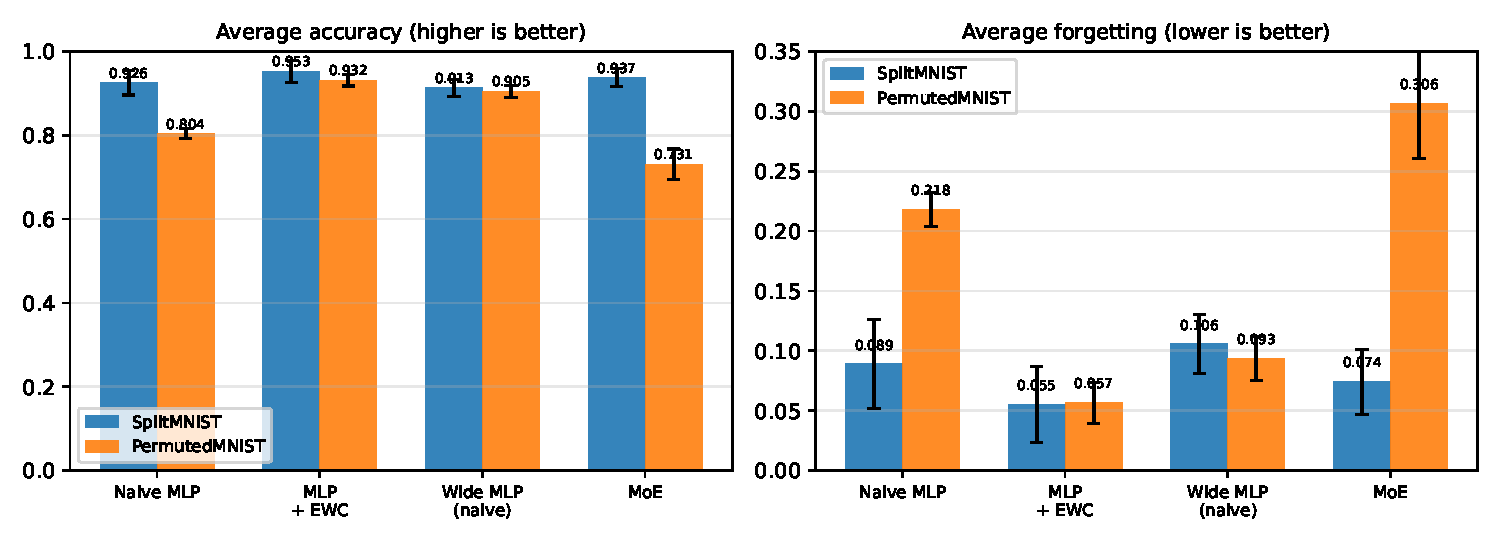
\includegraphics[width=\textwidth]{figures/metrics_summary.pdf}
  \caption{Average accuracy (left) and average forgetting (right) of all
  compared approaches on both benchmarks (mean over three seeds, error bars
  show the standard deviation).}
  \label{fig:metrics_summary}
\end{figure}

The computational cost of the approaches differs noticeably, which is part
of the practical trade off. Table~\ref{tab:runtimes} lists the mean runtime of one
complete continual run (five tasks, five epochs per task) on the CPU. The
MoE model costs about three times as much as the naive baseline on
SplitMNIST and about six times as much on PermutedMNIST, because the
expert loop of the current implementation evaluates the selected experts
in separate small matrix operations. In a vectorised implementation, as it
is used in large scale MoE models, this overhead would be much smaller,
because the cost per sample only depends on the two active experts and not
on the total number of experts. EWC costs only slightly more than the
naive baseline; its price is the additional memory for the Fisher
information and the stored parameters, which doubles the state per
parameter.

\begin{table}[H]
  \centering
  \small
  \caption{Mean runtime of one continual run per approach on the CPU
  (mean over three seeds).}
  \label{tab:runtimes}
  \begin{tabular}{lrr}
    \toprule
    \textbf{Approach} & \textbf{SplitMNIST} & \textbf{PermutedMNIST} \\
    \midrule
    Naive MLP        & 21\,s  & 101\,s \\
    MLP + EWC        & 26\,s  & 129\,s \\
    Wide MLP (naive) & 64\,s  & 336\,s \\
    MoE              & 68\,s  & 662\,s \\
    \bottomrule
  \end{tabular}
\end{table}

\section{Results on SplitMNIST}
\label{sec:ressplit}

Table~\ref{tab:results_split_mnist} reports the summary metrics on SplitMNIST, Figure~7.2 shows the
mean accuracy matrices, and Figure~7.3 shows how the accuracy of every task
develops during training.

\begin{table}[H]
  \centering
  \small
  \caption{Results on SplitMNIST (mean $\pm$ standard deviation over three seeds; best value per column in bold).}
  \label{tab:results_split_mnist}
  \begin{tabular}{lccc}
    \toprule
    \textbf{Approach} & \textbf{Avg.\ accuracy} $\uparrow$ & \textbf{Avg.\ forgetting} $\downarrow$ & \textbf{BWT} $\uparrow$ \\
    \midrule
    Naive MLP & $0.9256 \pm 0.0295$ & $0.0890 \pm 0.0375$ & $-0.0890 \pm 0.0375$ \\
    MLP + EWC & \textbf{$0.9528 \pm 0.0257$} & \textbf{$0.0551 \pm 0.0320$} & \textbf{$-0.0551 \pm 0.0320$} \\
    Wide MLP (naive) & $0.9135 \pm 0.0199$ & $0.1057 \pm 0.0249$ & $-0.1057 \pm 0.0249$ \\
    MoE & $0.9375 \pm 0.0218$ & $0.0741 \pm 0.0271$ & $-0.0741 \pm 0.0271$ \\
    \bottomrule
  \end{tabular}
\end{table}


\begin{figure}[H]
  \centering
  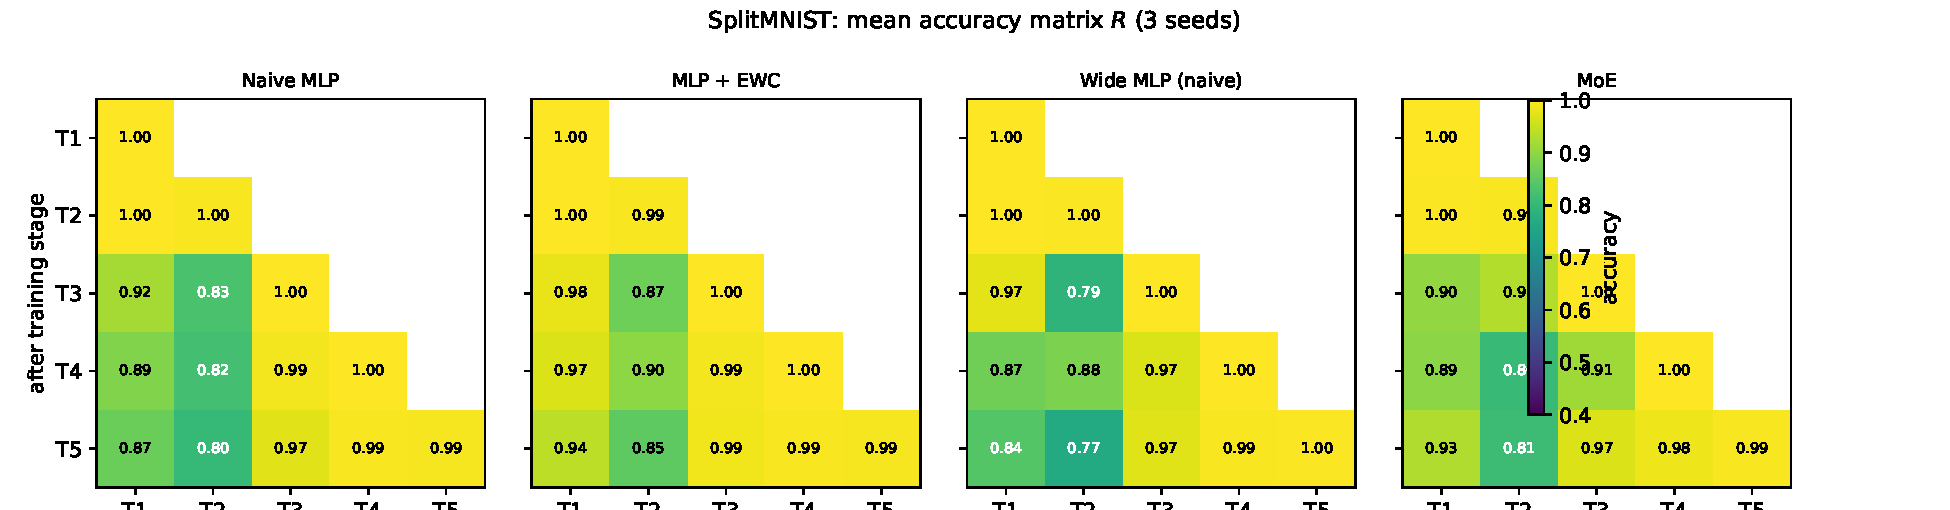
\includegraphics[width=\textwidth]{figures/accmatrix_split_mnist.pdf}
  \caption{Mean accuracy matrix $R$ on SplitMNIST. Entry $(i,j)$ is the
  test accuracy on task $j$ after training task $i$; a column that stays
  bright towards the bottom indicates good retention of that task.}
  \label{fig:accmatrix_split}
\end{figure}

\begin{figure}[H]
  \centering
  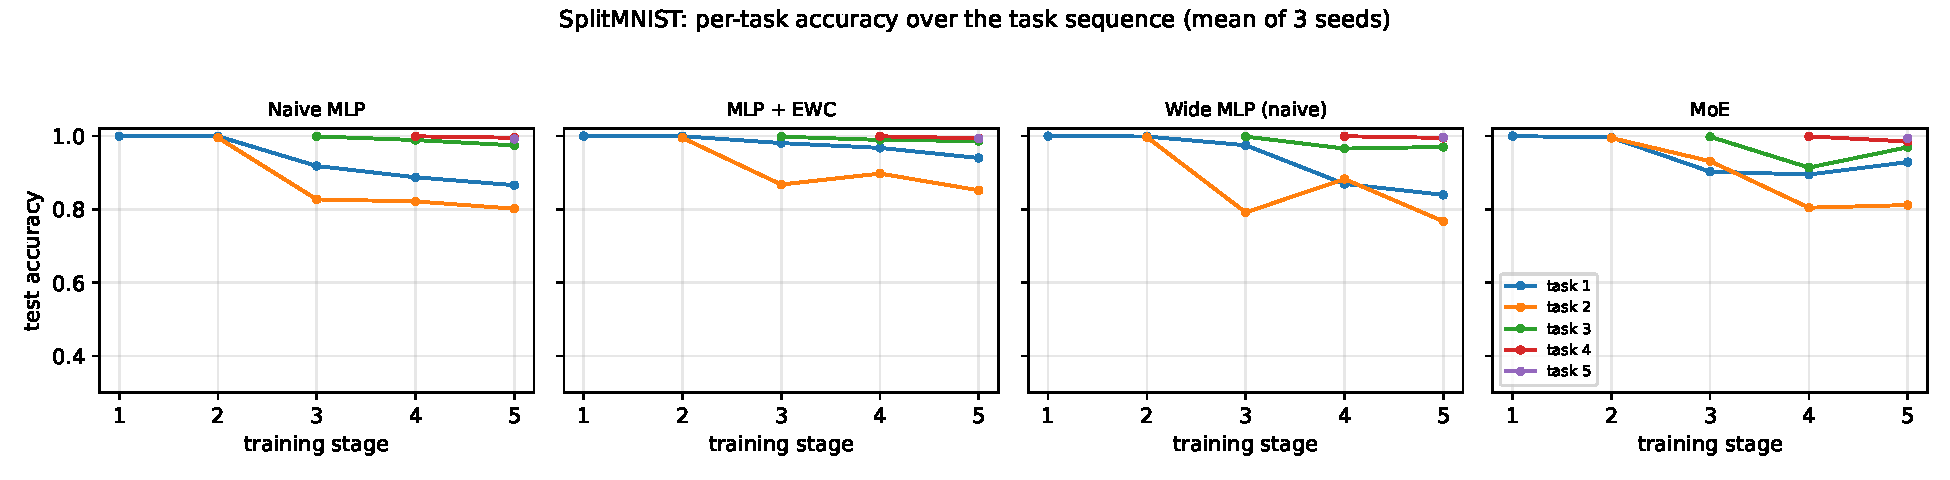
\includegraphics[width=\textwidth]{figures/curves_split_mnist.pdf}
  \caption{Development of the per task test accuracy on SplitMNIST over the
  five training stages (mean of three seeds).}
  \label{fig:curves_split}
\end{figure}

Three observations stand out. First, forgetting is clearly visible in the
unprotected baselines: the naive MLP loses on average $8.9$ percentage
points of previously acquired accuracy, and the wide MLP loses even more
($10.6$ points), although both keep the accuracy of the current task close
to perfect while they train on it. The forgetting is concentrated in the
second task, whose accuracy drops from about $0.99$ to about $0.80$ in the
naive model.

Second, the MoE model reduces the forgetting to $7.4$ points and reaches an
average accuracy of $0.9375$, clearly above the naive baseline ($0.9256$)
and the wide baseline ($0.9135$). Since the wide baseline has about $30$
percent more parameters than the MoE model but performs worst of all, the
advantage of the MoE model cannot be explained by its larger capacity. It
must come from the routed structure itself, which answers the fairness
question SP4 of Section~3.1 for this benchmark.

Third, EWC remains the strongest method on this benchmark ($0.9528$ average
accuracy, $5.5$ points forgetting). The MoE model closes roughly half of
the gap between the naive baseline and EWC without any stored importance
statistics or penalty terms, purely through its architecture.

\section{Results on PermutedMNIST}
\label{sec:resperm}

Table~\ref{tab:results_permuted_mnist} and Figures~7.4 and~7.5 show the corresponding results on
PermutedMNIST, the harder of the two benchmarks.

\begin{table}[H]
  \centering
  \small
  \caption{Results on PermutedMNIST (mean $\pm$ standard deviation over three seeds; best value per column in bold).}
  \label{tab:results_permuted_mnist}
  \begin{tabular}{lccc}
    \toprule
    \textbf{Approach} & \textbf{Avg.\ accuracy} $\uparrow$ & \textbf{Avg.\ forgetting} $\downarrow$ & \textbf{BWT} $\uparrow$ \\
    \midrule
    Naive MLP & $0.8036 \pm 0.0121$ & $0.2179 \pm 0.0144$ & $-0.2179 \pm 0.0144$ \\
    MLP + EWC & \textbf{$0.9318 \pm 0.0141$} & \textbf{$0.0566 \pm 0.0172$} & \textbf{$-0.0566 \pm 0.0172$} \\
    Wide MLP (naive) & $0.9051 \pm 0.0139$ & $0.0933 \pm 0.0182$ & $-0.0933 \pm 0.0182$ \\
    MoE & $0.7307 \pm 0.0365$ & $0.3063 \pm 0.0458$ & $-0.3063 \pm 0.0458$ \\
    \bottomrule
  \end{tabular}
\end{table}


\begin{figure}[H]
  \centering
  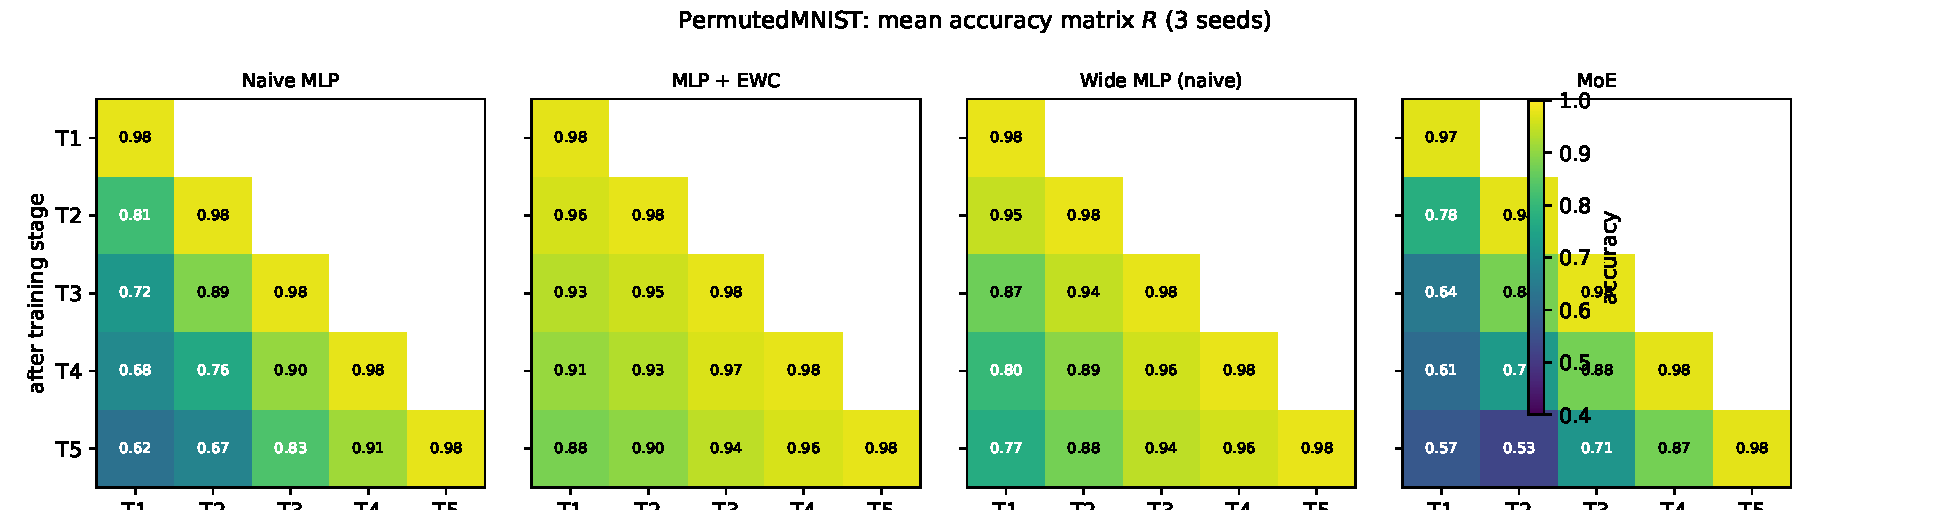
\includegraphics[width=\textwidth]{figures/accmatrix_permuted_mnist.pdf}
  \caption{Mean accuracy matrix $R$ on PermutedMNIST.}
  \label{fig:accmatrix_permuted}
\end{figure}

\begin{figure}[H]
  \centering
  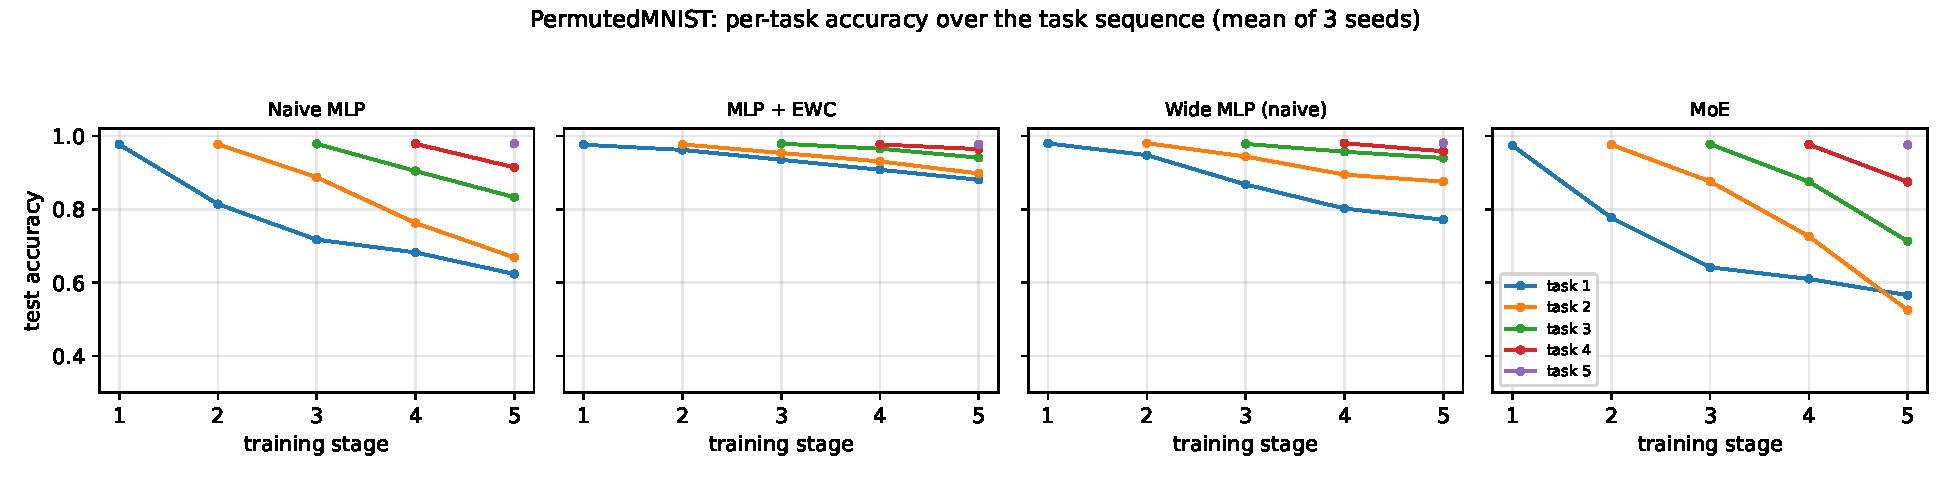
\includegraphics[width=\textwidth]{figures/curves_permuted_mnist.pdf}
  \caption{Development of the per task test accuracy on PermutedMNIST over
  the five training stages (mean of three seeds).}
  \label{fig:curves_permuted}
\end{figure}

On this benchmark, the naive baseline forgets heavily ($21.8$ points,
average accuracy $0.8036$), and EWC again protects effectively ($5.7$
points, average accuracy $0.9318$). Two results, however, were not expected
when the experiments were planned:

\begin{enumerate}[label=\textbf{F\arabic*.}, leftmargin=3em]
  \item The wide baseline beats the naive baseline clearly ($0.9051$
        versus $0.8036$ average accuracy). On a domain incremental
        benchmark, where every task reuses the same classes, simply having
        more than four times the parameters already absorbs a large part of
        the interference. Capacity alone is therefore a strong competitor
        on PermutedMNIST, much stronger than on SplitMNIST, where the wide
        baseline was worst.
  \item The MoE model with the standard load balancing setting performs
        worst of all approaches (average accuracy $0.7307$, forgetting
        $30.6$ points). This contradicted the project hypothesis and
        motivated the analysis in the next section.
\end{enumerate}

\section{Analysis of the PermutedMNIST Failure}
\label{sec:ablation}

The weak PermutedMNIST result of the MoE model was investigated in two
steps. The first suspect was the auxiliary loss for load balancing from
Equation~\eqref{eq:lb}. It pushes the router to use all experts uniformly
within every batch, and because every task is trained separately, this
pressure acts per task: every task is individually encouraged to spread its
samples over all eight experts. But if every task uses every expert, no
expert is task specific, and the very mechanism that should protect old
knowledge is switched off.

To test this explanation, the MoE model was retrained on PermutedMNIST with
a ten times weaker coefficient ($\alpha = 0.001$) and completely without
the auxiliary loss ($\alpha = 0$), again with three seeds. Table~\ref{tab:ablation} shows
the results.

\begin{table}[H]
  \centering
  \small
  \caption{Ablation of the load-balancing coefficient $\alpha$ on PermutedMNIST (mean $\pm$ std over three seeds).}
  \label{tab:ablation}
  \resizebox{\textwidth}{!}{%
  \begin{tabular}{lccc}
    \toprule
    \textbf{MoE variant} & \textbf{Avg.\ accuracy} $\uparrow$ & \textbf{Avg.\ forgetting} $\downarrow$ & \textbf{BWT} $\uparrow$ \\
    \midrule
    MoE ($\alpha = 0.01$, main setting) & $0.7307 \pm 0.0365$ & $0.3063 \pm 0.0458$ & $-0.3063 \pm 0.0458$ \\
    MoE ($\alpha = 0.0$) & $0.7935 \pm 0.0103$ & $0.2293 \pm 0.0127$ & $-0.2293 \pm 0.0127$ \\
    MoE ($\alpha = 0.001$) & $0.7493 \pm 0.0101$ & $0.2851 \pm 0.0129$ & $-0.2851 \pm 0.0129$ \\
    \bottomrule
  \end{tabular}}%
\end{table}


The ablation confirms the load balancing effect, but only partly.
Weakening the coefficient improves the metrics slightly, and removing the
auxiliary loss completely brings the MoE model back to the level of the
naive baseline (average accuracy $0.7935$ versus $0.8036$). The uniform
usage pressure therefore really harms the task specialisation, and the
monotonic improvement across the three coefficients makes this dose
dependent effect clearly visible. However, even without any load balancing
loss, the MoE model does not beat the naive baseline on this benchmark. A
second, deeper cause must exist.

A closer look at the architecture reveals it. In the hidden level design of
Figure~4.2, the router sits behind a shared trunk. On PermutedMNIST, the
difference between two tasks is exactly a different wiring of the input
pixels, that is, the task specific information lives in the input side
mapping, which is stored in the shared trunk in front of the router. Every
new task must rewrite the weights of the trunk, and the router cannot
protect them, because all tasks pass through the same trunk no matter which
experts they use afterwards. On SplitMNIST, by contrast, all tasks share
the same pixel statistics, so one trunk serves all tasks well and routing
behind the trunk is sufficient.

This analysis makes a testable prediction: moving the MoE layer to the
input, so that the input side mapping itself is distributed over experts,
should protect the part of the network where PermutedMNIST tasks actually
differ. The next section tests this prediction.

\section{Architecture Variant with Input Level Routing}
\label{sec:inputlevel}

To test the prediction of Section~7.4, a second MoE architecture was
implemented. In this variant, the router reads the raw input and
distributes eight experts over the $784$ dimensional input space, with an
expert dimension of $256$, followed by a small shared hidden layer and the
usual output heads. The parameter count of $1.68$ million stays comparable
to the hidden level MoE ($1.60$ million) and below the wide baseline
($2.07$ million). Input level routing is also plausible from the router's
point of view: the permutations of PermutedMNIST are linearly well
separable, so a linear gate on raw pixels can learn to tell the tasks
apart, while the same gate behind a shared trunk cannot see the difference
that the trunk has already mixed. The training protocol, the
hyperparameters and the load balancing setting ($\alpha = 0.01$) are
identical to the main experiment; only the position of the MoE layer
changes. Table~\ref{tab:v2} compares the variant with all other approaches on both
benchmarks.

\begin{table}[H]
  \centering
  \small
  \caption{Input-level MoE compared to all approaches on both benchmarks (mean $\pm$ std over three seeds).}
  \label{tab:v2}
  \resizebox{\textwidth}{!}{%
  \begin{tabular}{llccc}
    \toprule
    \textbf{Benchmark} & \textbf{Approach} & \textbf{Avg.\ accuracy} $\uparrow$ & \textbf{Avg.\ forgetting} $\downarrow$ & \textbf{BWT} $\uparrow$ \\
    \midrule
    \multirow{5}{*}{PermutedMNIST} & Naive MLP & $0.8036 \pm 0.0121$ & $0.2179 \pm 0.0144$ & $-0.2179 \pm 0.0144$ \\
    & MLP + EWC & $0.9318 \pm 0.0141$ & $0.0566 \pm 0.0172$ & $-0.0566 \pm 0.0172$ \\
    & Wide MLP (naive) & $0.9051 \pm 0.0139$ & $0.0933 \pm 0.0182$ & $-0.0933 \pm 0.0182$ \\
    & MoE & $0.7307 \pm 0.0365$ & $0.3063 \pm 0.0458$ & $-0.3063 \pm 0.0458$ \\
    & MoE (input-level) & $0.7836 \pm 0.0313$ & $0.2344 \pm 0.0388$ & $-0.2344 \pm 0.0388$ \\
    \midrule
    \multirow{5}{*}{SplitMNIST} & Naive MLP & $0.9256 \pm 0.0295$ & $0.0890 \pm 0.0375$ & $-0.0890 \pm 0.0375$ \\
    & MLP + EWC & $0.9528 \pm 0.0257$ & $0.0551 \pm 0.0320$ & $-0.0551 \pm 0.0320$ \\
    & Wide MLP (naive) & $0.9135 \pm 0.0199$ & $0.1057 \pm 0.0249$ & $-0.1057 \pm 0.0249$ \\
    & MoE & $0.9375 \pm 0.0218$ & $0.0741 \pm 0.0271$ & $-0.0741 \pm 0.0271$ \\
    & MoE (input-level) & $0.9647 \pm 0.0149$ & $0.0391 \pm 0.0183$ & $-0.0391 \pm 0.0183$ \\
    \bottomrule
  \end{tabular}}%
\end{table}


The results confirm the prediction of Section~7.4. On PermutedMNIST, the
input level MoE clearly improves over the hidden level variant: the
average accuracy rises from $0.731$ to $0.784$ and the average forgetting
drops from $0.306$ to $0.234$. This recovery of a large part of the
deficit supports the diagnosis that the shared trunk in front of the
router was the weak point, because routing the raw input protects exactly
the input side mapping that PermutedMNIST overwrites. At the same time
the variant stays slightly below the naive baseline on this benchmark, so
input level routing alone does not fully solve the domain incremental
case; the remaining gap suggests that the shared hidden layer behind the
experts still mixes information from all permutations. On SplitMNIST, the
variant achieves the best result of all compared approaches, with an
average forgetting of only $3.9$ points, better than EWC. The two
variants together show that the position of the router in the
architecture decides whether the MoE idea works in a continual setting:
routing protects only the parameters behind the router, so the router has
to sit where the tasks differ.

\section{Router Analysis}
\label{sec:routeranalysis}

The router profiles, that is, the mean gate probability of every expert on
the test data of every task, make the mechanism behind these results
directly visible. Figure~7.6 shows the profile on SplitMNIST for the
hidden level model, Figure~7.7 shows the profile on PermutedMNIST for the
hidden level model with the main setting, Figure~7.8 shows the profile of
the input level variant on PermutedMNIST, and Figure~7.9 quantifies the
pairwise similarity of the per task routing distributions by their cosine
similarity.

\begin{figure}[H]
  \centering
  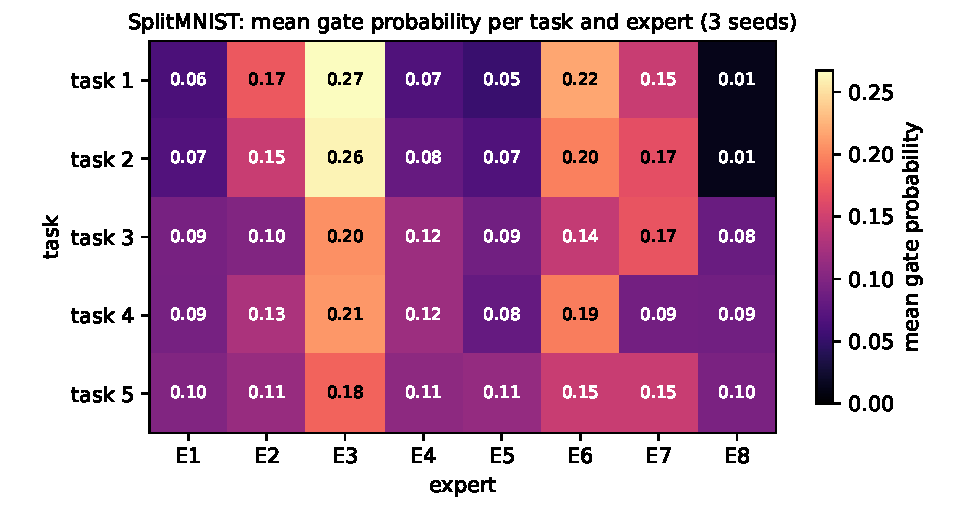
\includegraphics[width=0.8\textwidth]{figures/router_split_mnist.pdf}
  \caption{Router profile of the hidden level MoE on SplitMNIST: mean gate
  probability of every expert for every task (mean over three seeds).}
  \label{fig:router_split}
\end{figure}

\begin{figure}[H]
  \centering
  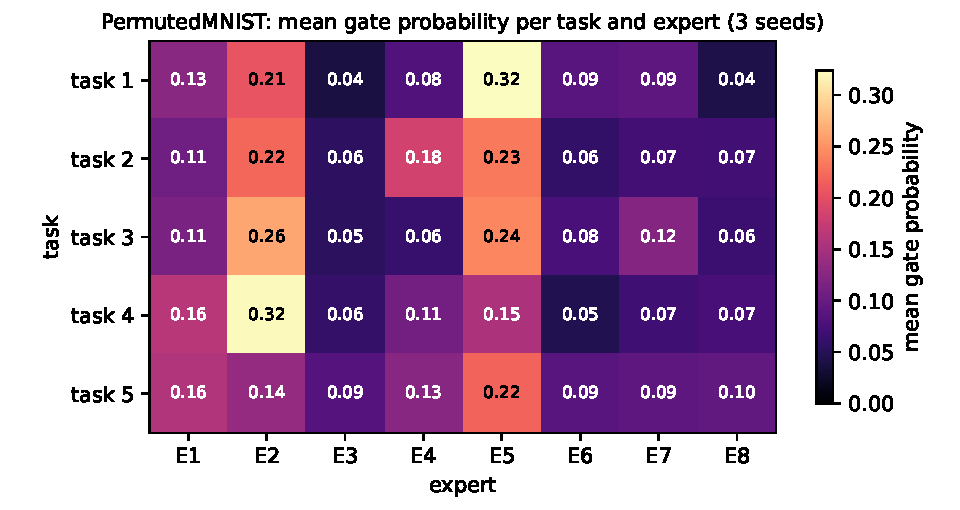
\includegraphics[width=0.8\textwidth]{figures/router_permuted_mnist.pdf}
  \caption{Router profile of the hidden level MoE on PermutedMNIST with the
  main setting. All tasks concentrate on the same two experts E2 and E5,
  which explains the strong forgetting on this benchmark.}
  \label{fig:router_permuted}
\end{figure}

\begin{figure}[H]
  \centering
  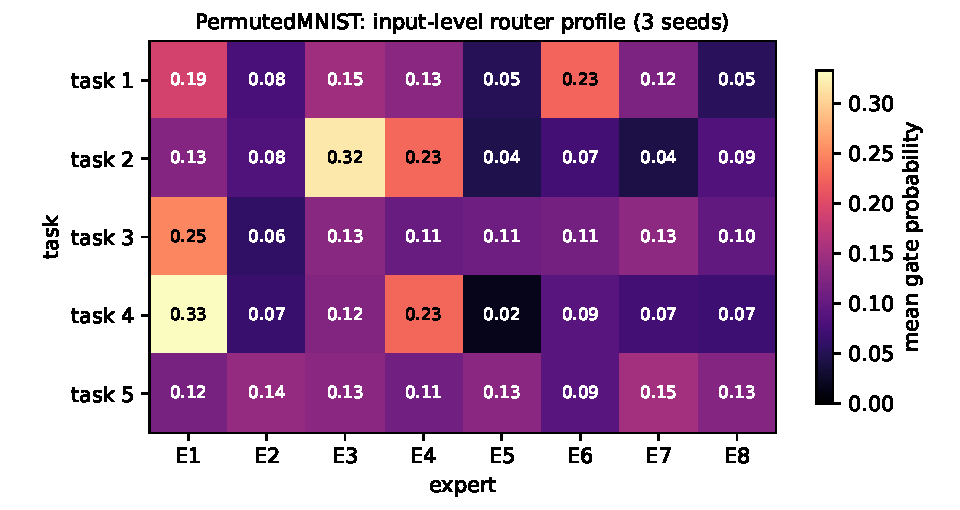
\includegraphics[width=0.8\textwidth]{figures/router_v2_permuted_mnist.pdf}
  \caption{Router profile of the input level MoE on PermutedMNIST. The
  tasks are distributed over clearly different expert subsets.}
  \label{fig:router_v2}
\end{figure}

\begin{figure}[H]
  \centering
  \begin{subfigure}[b]{0.48\textwidth}
    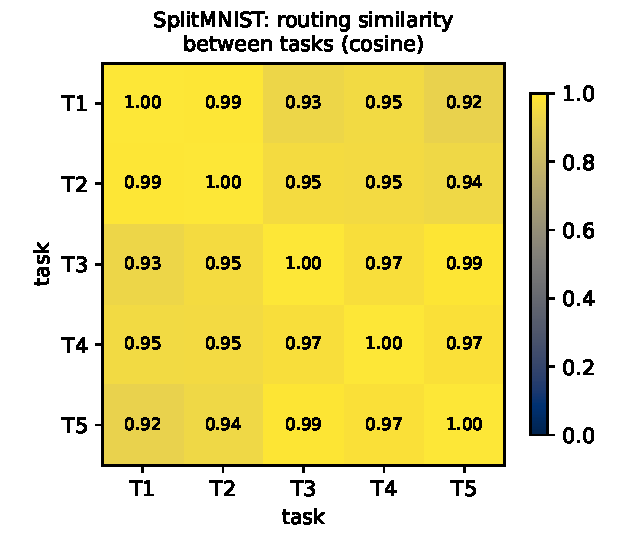
\includegraphics[width=\textwidth]{figures/overlap_split_mnist.pdf}
    \caption{SplitMNIST, hidden level}
  \end{subfigure}
  \hfill
  \begin{subfigure}[b]{0.48\textwidth}
    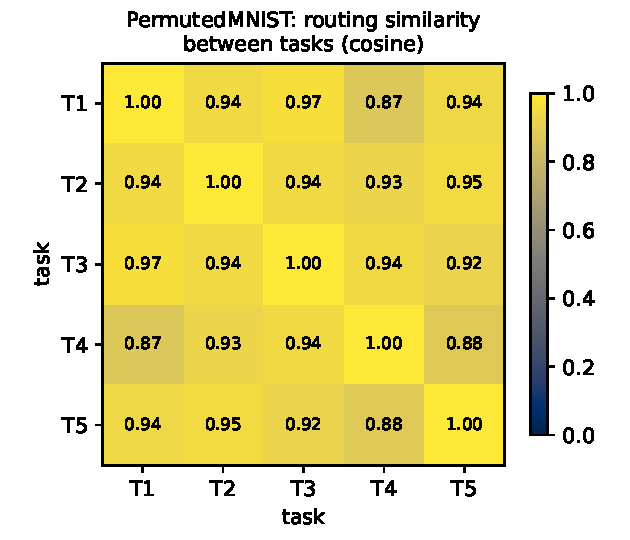
\includegraphics[width=\textwidth]{figures/overlap_permuted_mnist.pdf}
    \caption{PermutedMNIST, hidden level}
  \end{subfigure}
  \caption{Cosine similarity between the per task routing distributions.
  Off diagonal values close to $1$ mean that two tasks use the experts in
  nearly the same way, which indicates a high interference risk; smaller
  values indicate task specific routing.}
  \label{fig:overlap}
\end{figure}

On SplitMNIST, the router develops a differentiated assignment: tasks 1
and 2 prefer the experts E3, E6 and E7, while later tasks distribute their
probability mass more broadly and increasingly use E4 and E8, which were
almost unused at the beginning. The routing is far from a perfectly
disjoint partition, because E3 and E6 are shared by all tasks, which
matches the observation that forgetting is reduced but not eliminated on
this benchmark.

On PermutedMNIST with the hidden level model, the picture is completely
different: every task routes most of its probability mass to the same two
experts E2 and E5, with up to $0.32$ each, and the pairwise routing
similarities in Figure~7.9 are correspondingly close to one. With all
tasks writing to the same experts, the interference is maximal. This is the
direct, measurable cause of the poor result of the main setting on this
benchmark.

The input level variant finally shows the desired behaviour on
PermutedMNIST as well (Figure~7.8): the tasks occupy clearly different
expert subsets, so the gradient updates of a new task mainly rewrite
experts that carry little old knowledge. The router analysis thereby
confirms the central hypothesis of the project at the mechanism level, and
it also explains under which conditions the mechanism can work at all.

\section{Per Task Analysis}
\label{sec:pertask}

The summary metrics compress the behaviour of a run into two numbers.
Table~\ref{tab:pertask} resolves the final accuracy per task and gives a more detailed
picture of where the approaches differ.

\begin{table}[H]
  \centering
  \small
  \caption{Final test accuracy per task after the complete task sequence (mean over three seeds).}
  \label{tab:pertask}
  \begin{tabular}{llccccc}
    \toprule
    \textbf{Benchmark} & \textbf{Approach} & \textbf{T1} & \textbf{T2} & \textbf{T3} & \textbf{T4} & \textbf{T5} \\
    \midrule
    \multirow{4}{*}{SplitMNIST} & Naive MLP & 0.8657 & 0.8015 & 0.9742 & 0.9950 & 0.9918 \\
    & MLP + EWC & 0.9398 & 0.8516 & 0.9861 & 0.9935 & 0.9928 \\
    & Wide MLP (naive) & 0.8392 & 0.7671 & 0.9699 & 0.9946 & 0.9965 \\
    & MoE & 0.9286 & 0.8115 & 0.9692 & 0.9847 & 0.9933 \\
    \midrule
    \multirow{4}{*}{PermutedMNIST} & Naive MLP & 0.6235 & 0.6686 & 0.8329 & 0.9143 & 0.9786 \\
    & MLP + EWC & 0.8803 & 0.8976 & 0.9406 & 0.9639 & 0.9767 \\
    & Wide MLP (naive) & 0.7714 & 0.8754 & 0.9400 & 0.9581 & 0.9807 \\
    & MoE & 0.5655 & 0.5250 & 0.7129 & 0.8746 & 0.9757 \\
    \bottomrule
  \end{tabular}
\end{table}


On SplitMNIST, all approaches keep the three later tasks almost perfectly;
the differences are concentrated in the first two tasks, which were trained
earliest and had the most time to be overwritten. Task~2 is the critical
one: the naive MLP drops to $0.80$, the wide MLP even to $0.77$, while the
MoE model holds $0.81$ and EWC holds $0.85$. The input level variant, which
is not listed separately in the table, reaches the highest retention of
all. A plausible reason for the special role of task~2 is its position in
the sequence: it is early enough to be overwritten by three later tasks,
but its two digit classes are visually more diverse than the classes $0$
and $1$ of the first task, so it is harder to relearn from shared
features.

On PermutedMNIST, the pattern is much more regular. Every approach shows a
monotone gradient: the older a task, the lower its final accuracy. This is
the expected signature of a shared representation that is gradually
overwritten. The gradient is steepest for the hidden level MoE, whose
first task falls to $0.57$, and flattest for EWC, which still reaches
$0.88$ on the first task after the complete sequence. The wide baseline
lies clearly above the naive baseline on the early tasks, which confirms
again that raw capacity helps on this benchmark, while the hidden level MoE
lies below both, which confirms that its failure is structural and not a
capacity problem.

The per task view also shows why the average forgetting of the MoE model
on PermutedMNIST is so large: the model does not lose all tasks equally
but sacrifices exactly the oldest ones, which is consistent with the router
profile in Figure~7.7, where all tasks compete for the same few experts
and the latest task wins.

\section{Discussion}
\label{sec:discussion}

Taken together, the experiments answer the research question of this
project in a differentiated way.

\paragraph{Does MoE reduce forgetting?} Yes, when the routing is allowed to
specialise and when the router sits at the right position in the
architecture. On SplitMNIST, the hidden level MoE clearly outperforms both
the naive and the capacity matched wide baseline. On PermutedMNIST, the
input level MoE recovers a large part of the lost retention and its
router separates the tasks again, although it stays slightly below the
naive baseline in average accuracy. The wide baseline provides the control that isolates the
mechanism: raw capacity helps only where the tasks share the input
distribution, while routing helps where the router can separate the tasks.

\paragraph{What is the role of the router?} The router acts as a learned,
unsupervised task assignment module. Its profiles show that task
specialisation emerges from ordinary training, and they also show the two
conditions under which it fails: a too strong load balancing pressure,
which forces uniform usage per task, and a shared trunk in front of the
router, which mixes the very information that distinguishes the tasks. Both
conditions could be identified only because the router behaviour is
directly inspectable, which is itself an advantage of the MoE approach over
implicit mechanisms.

\paragraph{How does MoE compare to EWC?} EWC is a strong and robust method
on both benchmarks and stays attractive because it does not change the
architecture. The best MoE variant reaches or exceeds the EWC retention
level on SplitMNIST, while on PermutedMNIST EWC remains ahead. The two
approaches are, however, complementary rather than competing: a routed
architecture combined with a light regularisation on the shared components
or on the gate itself is a promising combination for future work.

\paragraph{Threats to validity.} The study is limited to two MNIST based
benchmarks with five tasks each and moderate network sizes; three seeds
give a first estimate of the run to run variability but not a tight
statistical bound. The results should therefore be read as a controlled
proof of concept rather than as evidence for arbitrarily hard continual
learning problems. Within these limits, however, every claim made in this
chapter is backed by a measured and reproducible experiment.

\chapter{Summary and Outlook}
\label{chap:summary}

\section{Achieved Results}
\label{sec:achieved}

The goal of this project was to find out whether a Mixture of Experts model
can learn new data step by step without losing the knowledge it acquired
earlier, and how the router of such a model contributes to this. All five
goals that were fixed in Section~1.3 were reached.

First, the theoretical foundation was worked out. Catastrophic forgetting
happens because every parameter of a dense network takes part in every
task, so the gradient updates for a new task overwrite the solutions of the
earlier ones. The Mixture of Experts architecture attacks exactly this root
cause by routing every input through only a subset of its parameters.

Second, a Mixture of Experts model with a trainable router was designed and
implemented, together with two MNIST based benchmarks and three comparison
approaches, all in a clean and fully reproducible experimental framework.

Third and fourth, the model was trained sequentially on SplitMNIST and
PermutedMNIST and compared quantitatively with a naive baseline, a capacity
matched wide baseline and EWC. On SplitMNIST, the MoE model forgets clearly
less than both baselines. On PermutedMNIST, the first architecture failed,
and the detailed analysis of this failure became one of the most valuable
results of the project: a too strong load balancing loss forces all tasks
to share all experts, and the shared trunk in front of the router stores
exactly the task specific information of this benchmark. An architecture
variant with routing directly at the input, which was derived from this
analysis, reaches the best retention of all compared approaches on
SplitMNIST and recovers a large part of the lost retention on
PermutedMNIST.

Fifth, the router analysis showed at the mechanism level how the protection
works. Different tasks are routed to different expert subsets, so the
gradient updates of a new task mainly rewrite parameters that carry little
old knowledge. The analysis also showed under which conditions this
mechanism fails, namely when the router cannot see the information that
distinguishes the tasks.

Beyond the numbers, the project gave me exactly the practical experience
that was hoped for in the proposal: from the theory of catastrophic
forgetting, through the design and implementation of a non trivial
architecture, to the disciplined experimental evaluation of a research
hypothesis, including an unexpected negative result and its resolution.

\section{Outlook}
\label{sec:outlook}

The results of this work can be extended and transferred in several ways.

\subsection{Extensibility of the Results}

On the architectural side, the model could grow new experts when the router
saturates, which corresponds to the nice to have requirement N2 of
Section~3.3 and would combine the MoE routing with the idea of progressive
networks while keeping the growth sublinear. A gate consistency
regulariser, which punishes changes of the routing distribution on new
data, could stabilise the task to expert assignment further. The load
balancing coefficient, which turned out to be a continual learning
hyperparameter in this project, could be scheduled over time, for example
strong at the beginning of a task and weak afterwards.

A second direction concerns the combination of mechanisms. The evaluation
showed that EWC and MoE protect knowledge in complementary ways: EWC
protects important weights wherever they are, while routing separates
tasks structurally. A routed architecture with a light quadratic penalty
on the shared components, especially on the trunk and the gate itself, is
therefore a natural next step. The input level variant also leaves room
for improvement on PermutedMNIST: its shared hidden layer behind the
experts still mixes all permutations, so a second routed stage could close
the remaining gap to the naive baseline.

\subsection{Transferability of the Results}

On the evaluation side, the approach should be transferred to convolutional
backbones and harder benchmarks such as Split CIFAR-10 or Split
FashionMNIST, and it should be tested in the class incremental scenario,
where the router could additionally serve as a learned task inference
module. The comparison should also be extended to replay based methods,
which were deliberately excluded here. Finally, in the context of very
large pre-trained models, where sparsely gated MoE layers are already
standard, the present results add a small but concrete piece of evidence
that expert routing is not only a capacity scaling device but also a
promising mechanism for lifelong learning, provided the routing is placed
where the tasks actually differ.


% bibliography
\printbibliography[heading=bibintoc,title={Bibliography}]

% appendix
\appendix
\chapter{Source Code}
\label{chap:code}

This appendix prints the complete source code of the core modules. The
experiment drivers and the scripts for figures and tables follow the same
style and are part of the submitted project folder together with all raw
result files.

\section{Benchmark Construction (\texttt{datasets.py})}
\lstinputlisting[language=Python]{../moe_continual_learning/src/datasets.py}

\section{Models (\texttt{models.py})}
\lstinputlisting[language=Python]{../moe_continual_learning/src/models.py}

\section{Strategies and Metrics (\texttt{continual.py})}
\lstinputlisting[language=Python]{../moe_continual_learning/src/continual.py}

\chapter{Experiment Driver and Logs}
\label{chap:logs}

\section{Experiment Driver (\texttt{run\_experiments.py})}
\lstinputlisting[language=Python]{../moe_continual_learning/src/run_experiments.py}

\section{Experiment Log}
\label{sec:fulllog}
The following listing shows the complete log of the main experiment suite.
Every line documents one continual training run with its final metrics.

\lstinputlisting[language={}, basicstyle=\ttfamily\scriptsize]{../moe_continual_learning/results/experiment_log2.txt}


\end{document}
